%!TEX encoding = UTF-8 Unicode
\documentclass[
    fontsize=12pt,
    headings=small,
    parskip=half,           % Ersetzt manuelles setzten von parskip/parindent.
    bibliography=totoc,
    numbers=noenddot,       % Entfernt den letzten Punkt der Kapitelnummern.
    open=any               % Kapitel kann auf jeder Seite beginnen.
   %,final                   % Entfernt alle todonotes und den Entwurfstempel.
    ]{scrreprt}

% ===================================Praeambel==================================

% Kodierung, Sprache, Patches {{{
\usepackage[T1]{fontenc}    % Ausgabekodierung; ermoeglicht Akzente und Umlaute
                            %  sowie korrekte Silbentrennung.
\usepackage[utf8]{inputenc} % Erlaub die direkte Eingabe spezieller Zeichen.
                            %  Utf8 muss die Eingabekodierung des Editors sein.
\usepackage[ngerman]{babel} % Deutsche Sprachanpassungen (z.B. Ueberschriften).
\usepackage{microtype}      % Optimale Randausrichtung und Skalierung.
\usepackage[
    autostyle,
    ]{csquotes}             % Korrekte Anfuehrungszeichen in der Literaturliste.
\usepackage{fixltx2e}       % Patches fuer LaTeX2e.
\usepackage{scrhack}        % Verhindert Warnungen mit aelteren Paketen.
\usepackage[
  newcommands
]{ragged2e}                 % Verbesserte \ragged...Befehle
\PassOptionsToPackage{
  hyphens
}{url}                      % Sorgt für URL-Umbrueche in Fusszeilen u. Literatur
% }}}

% Schriftarten {{{
\usepackage{mathptmx}       % Times; modifies the default serif and math fonts
\usepackage[scaled=.92]{helvet}% modifies the sans serif font
\usepackage{courier}        % modifies the monospace font
% }}}

% Biblatex {{{
\usepackage[
    style=alphabetic,
    backend=bibtex,
    %backref=true
    ]{biblatex}             % Biblatex mit alphabetischem Style und biber.
\bibliography{literature}      % Dateiname der bib-Datei.
%\addbibresource{literature.bib}
\DeclareFieldFormat*{title}{
    \mkbibemph{#1}}         % Make titles italics
% }}}

% Dokument- und Texteinstellungen {{{
\usepackage[
    a4paper,
    margin=2.54cm,
    marginparwidth=2.0cm,
    footskip=1.0cm
    ]{geometry}             % Ersetzt 'a4wide'.
\clubpenalty=10000          % Keine Einzelzeile am Beginn eines Paragraphen
                            %  (Schusterjungen).
\widowpenalty=10000         % Keine Einzelzeile am Ende eines Paragraphen
\displaywidowpenalty=10000  %  (Hurenkinder).
\usepackage{floatrow}       % Zentriert alle Floats.
\usepackage{ifdraft}        % Ermoeglicht \ifoptionfinal{true}{false}
\pagestyle{plain}           % keine Kopfzeilen
% \sloppy                    % großzügige Formatierungsweise
\deffootnote{1em}{1em}{
  \thefootnotemark.\ }      % Verbessert Layout mehrzeiliger Fußnoten

\makeatletter
\AtBeginDocument{%
    \hypersetup{%
        pdftitle = {Masterarbeit Datenschutzfreundliche Speicherung},
        pdfauthor  = \@author,
    }
}
\makeatother
% }}}

% Weitere Pakete {{{
\usepackage{graphicx}       % Einfuegen von Graphiken.
\usepackage{tabu}           % Einfuegen von Tabellen.
\usepackage{multirow}       % Tabellenzeilen zusammenfassen.
\usepackage{multicol}       % Tabellenspalten zusammenfassen.
\usepackage{booktabs}       % Schönere Tabellen (\toprule\midrule\bottomrule).
\usepackage[nocut]{thmbox}  % Theorembox bspw. fuer Angreifermodell.
\usepackage{amsmath}        % Erweiterte Handhabung mathematischer Formeln.
\usepackage{amssymb}        % Erweiterte mathematische Symbole.
\usepackage{rotating}
\usepackage[
    printonlyused
    ]{acronym}              % Abkuerzungsverzeichnis.
\usepackage[
    colorinlistoftodos,
    textsize=tiny,          % Notizen und TODOs - mit der todonotes.sty von
    \ifoptionfinal{disable}{}%  Benjamin Kellermann ist das Package "changebar"
    ]{todonotes}            %  bereits integriert.
\usepackage[
    breaklinks,
    hidelinks,
    pdfdisplaydoctitle,
    pdfpagemode = {UseOutlines},
    pdfpagelabels,
    ]{hyperref}             % Sprungmarken im PDF. Laed das URL Paket.
\urlstyle{rm}           % Entfernt die Formattierung von URLs.
%\usepackage{breakurl}
%\def\UrlBreaks{\do\/\do-}
\usepackage{listings}       % Spezielle Umgebung für...
    \lstset{                %  ...Quelltextformatierung.
        language=C,
        breaklines=true,
        breakatwhitespace=true,
        frame=L,
        captionpos=b,
        xleftmargin=6ex,
        tabsize=4,
        numbers=left,
        numberstyle=\ttfamily\footnotesize,
        basicstyle=\ttfamily\footnotesize,
        keywordstyle=\bfseries\color{green!50!black},
        commentstyle=\itshape\color{magenta!90!black},
        identifierstyle=\ttfamily,
        stringstyle=\color{orange!90!black},
        showstringspaces=false,
        }
        
%===============================================================================


\usepackage{color}
\usepackage[most]{tcolorbox}
\definecolor{tbc-foreground}{rgb}{1,1,1}
\definecolor{tbc-background}{rgb}{0,0,.5}

\usepackage{pgfplots}
\usepackage{pgf-pie}

% Command for comments on questions or notes for supervisors
\newcommand{\tbc}[1]{
  \begin{tcolorbox}[
     enhanced jigsaw, % needed to really the frame off!
     colback=tbc-background, 
     coltext=tbc-foreground, 
     sharp corners, % no rounded corners
     boxrule=0pt % frame off 
  ]
    #1
  \end{tcolorbox}
}

% ===================================Dokument===================================

\title{Datenschutzfreundliche Speicherung\\unternehmensinterner Überwachungsdaten mittels\\Pseudonymisierung und kryptographischer\\Schwellwertschemata}
\author{Tom Petersen}
% \date{01.01.2015} % falls ein bestimmter Tag eingesetzt werden soll, einfach
                    %  diese Zeile aktivieren

\begin{document}

% ================================Deckblatt-Muster==============================
\newpage
\thispagestyle{empty}
% \addcontentsline{toc}{chapter}{Muster des Deckblatts}
\begin{titlepage}% {{{
\includegraphics[width=6.8cm]{./img/up-uhh-logo-u-2010-u-farbe-u-rgb.pdf}
\begin{center}\Large
	% Universität Hamburg \par
	% Fachbereich Informatik
	\vfill
	Masterarbeit
	\vfill
	\makeatletter
	{\Large\textsf{\textbf{\@title}}\par}
	\makeatother
	\vfill
	vorgelegt von
	\par\bigskip
	\makeatletter
	{\@author} \par
	\makeatother
	geb. am 13. Dezember 1990 in Hannover\par
	Matrikelnummer 3659640 \par
	Studiengang Informatik
	\vfill
	\makeatletter
	eingereicht am {\@date}
	\makeatother
	\vfill
	Betreuer: Dipl.-Inf. Ephraim Zimmer\par
	Erstgutachter: Prof. Dr. Hannes Federrath \par
	Zweitgutachter: Prof. Dr. Mathias Fischer\par
\end{center}
\ifoptionfinal{}{
	\begin{tikzpicture}[remember picture, overlay]
	    \node[draw, red, font=\ttfamily\bfseries\Huge, xshift=50mm, yshift=228mm,
	        rotate=340, text centered, text width=8cm, very thick, rounded
	        corners=4mm] at (current page.south) {Entwurf vom \today};
	\end{tikzpicture}}
\end{titlepage}% }}}

% ================================Content==============================

\pagenumbering{gobble}

\chapter*{Aufgabenstellung}

Die technologiegestützte Bekämpfung von Insider-Angriffen im Unternehmenskontext basiert aktuell häufig auf der Analyse des Nutzerverhaltens einzelner Mitarbeiter und der Erkennung von Abweichungen zum erwarteten Normalverhalten. Diese sogenannte Anomalieerkennung benötigt umfassende Überwachungsdaten aller digitalen Endgeräte und Datenkommunikationssysteme zur Erstellung und eindeutigen Zuordnung von Nutzerprofilen. Dabei entsteht ein Konflikt mit dem Datenschutz der Mitarbeiter, da die Erhebung, Verarbeitung und Speicherung von Überwachungsdaten einen schweren Eingriff in die Privatsphäre und die informationelle Selbstbestimmung der Mitarbeiter darstellt. Um diesen Konflikt zu lösen, können auf der einen Seite Datenschutztechniken eingesetzt werden, die den unmittelbaren Personenbezug gesammelter Daten entfernen. Auf der anderen Seite kann mithílfe von Kryptographie die Rückgewinnung des Personenbezugs im Verdachtsfall und unter der Voraussetzung einer mehrseitigen Kollaboration ermöglicht werden.

Das Ziel der Masterarbeit ist die konzepzionelle Erarbeitung einer solchen datenschutzfreundlichen und mehrseitig sicheren Erhebung, Verarbeitung und Speicherung von Überwachungsdaten sowie die prototypische Implementierung auf Basis eines Security Information Event Management Systems. Dabei sollen insbesondere die folgenden Punkte bearbeitet werden:

\begin{itemize}
  \item Wie ist der aktuelle Stand sowohl der Technik als auch der Wissenschaft im Bereich der Pseudonymisierung und der kryptographischen Schwellwertschemata?
  \item An welcher Stelle des konzipierten Systems können die Überwachungsdaten entsprechend des Datenschutzes und der späteren möglicherweise erforderlichen Rückgewinnung des Personenbezugs verarbeitet werden und welche Auswirkungen können entstehen?
  \item Wie und an welcher Stelle muss das Schlüsselmanagement der benötigten kryptographischen Funktionen erfolgen?
  \item Welche Alternativen gibt es neben der Pseudonymisierung und den kryptographischen Schwellwertschemata zur Lösung des genannten Zielkonflikts und wie können diese in das Konzept und die prototypische Implementierung integriert werden?
\end{itemize}

\listoftodos

\chapter*{Zusammenfassung}

\todo{TBW}

- Insiderangriffe
- Zielkonflikt: Anomalieerkennung vs. Arbeitnehemrdatenschutz
- Zusammenspiel von Pseudonymen und kryptogrpahischen SChwellwerrtschema (Suchproblem)
- Ausprägungen/Eigenschaften
- abstrakter Systementwurf und Implementierung/Evaluation eines (erweiterbaren) Prototypen (basierend auf SIEM-system)
- Implementierung Schwellwertschema

\tableofcontents

\newpage
\pagenumbering{arabic}

\chapter{Einführung}

\label{cha_introduction}

% Drei-Projekt erwähnen? Oder nur allgemeine Informationen entnehmen?



%- Insiderangriffe 

%- SIEM-Systeme in aktueller Form keine adäquate Lösung

%- Datenschutzrecht Arbeitnehmer

%- Mögliche Lösung: Pseudonymisierung und Schwellwertschemata mit verteilten Schlüsseln

%- Spannungsfeld Aufdeckbarkeit und Datenschutz

\todo{
Wo passen Abschnitte zu folgenden Stichworten hin?
- Verschiedene Datenarten: Identifizierend, Traffic, nicht relevant, ...
- Grundlegende Definition Insiderangriff
}

Liest man von erfolgreichen Angriffen auf Unternehmensnetzwerke, so ist die implizite Annahme von außenstehenden, unternehmensfremden Angreifern weit verbreitet. Doch häufig sind die Angreifer bereits im Netzwerk ansässig. Es handelt sich um (ehemalige) Mitarbeiter oder zumindest Personen mit legitimem Zugriff auf das Netzwerk, wie Geschäftspartnern oder Kunden. Hierbei geht es keineswegs lediglich um Einzelfälle. 

In dem \textit{IBM Cyber Security Intelligence Report} von 2015 werden 55\% der Angriffe als aus dem internen Netz stammend angegeben \cite{ibm2015}. Zu beachten ist allerdings, dass nicht nur mit Absicht ausgeführte Angriffe hierunter erfasst wurden, sondern auch unbeabsichtigte wie das versehentliche Veröffentlichen schützenswerter Kundendaten.

Auch der Branchenverband bitkom führt in seiner \textit{Spezialstudie Wirtschaftsschutz} aus dem Jahr 2016 nach einer Befragung von über 1000 Unternehmen aus, dass etwa 60\% der erfolgten Handlungen aus dem Bereich Datendiebstahl, Industriespionage oder Sabotage durch (ehemalige) Mitarbeiter erfolgten \cite{bitkom2016}.

\todo{Schadenshöhe (siehe Antrag)?}

Auch wenn die genauen Zahlen aufgrund von unterschiedlichen Annahmen und der in diesem Bereich nicht zu vernachlässigenden Dunkelziffer\footnote{
	Insbesondere die Angst vor Imageschäden, die auch in der \textit{Spezialstudie Wirtschaftsschutz} erwähnt wird, könnte ein Grund für das Geheimhalten von Vorfällen sein.
} mit Vorsicht zu betrachten sind, so geben sie doch Hinweise darauf, dass Angriffe von Innentätern weit verbreitet sind und ein hohes Schadenspotenzial aufweisen. Die Erkennung und Verhinderung solcher Angriffe sollte daher ein wichtiger Teil des IT-Sicherheitskonzepts eines Unternehmens sein.

Zur Erkennung von Angriffen in Netzwerken können SIEM-Systeme eingesetzt werden (siehe Abschnitt \ref{cha_siem}). Diese sind jedoch in erster Linie auf das Erkennen von externen Angriffen ausgelegt und in ihrer derzeitigen Form kaum sinnvoll für das Erkennen von Innentätern zu nutzen. \todo{EZ: Warum nicht? Einige werben damit, Innentaeter erkennen zu koennen, z.B. IBM QRadar} \\
Hierfür würden zusätzliche Datenquellen und Erkennungslogiken nötig sein.\todo{EZ: Warum? Welche?} 
Zusätzlich spielen auch  datenschutzrechtliche Bedenken im Bezug auf das Sammeln von großen Datenmengen über Mitarbeiter des eigenen Unternehmens hier eine entscheidende Rolle. Details hierzu sind im folgenden Kapitel \ref{cha_employee_privacy} zu finden.

Ein Ansatz, der diese Bedenken ausräumen oder zumindest lindern könnte, ist die Nutzung von Pseudonymen bei der Datenerfassung (siehe Abschnitt \ref{cha_pseudonym}). Anstatt direkt identifizierende Merkmale eines Arbeitnehmers abzuspeichern, werden diese Merkmale durch ein Pseudonym ersetzt. Eine Liste dieser Ersetzungen wird verschlüsselt abgelegt. Im Fall eines Angriffs durch einen Innentäter kann die Liste entschlüsselt werden und relevante Ereignisse de-pseudonymisiert, also ihrem ursprünglichen Verursacher wieder zweifelsfrei zugeordnet, werden.\\
Um die Entschlüsselung nicht einzelnen (möglicherweise bösartig agierenden) Personen zu ermöglichen, können sogenannte Schwellwertschemata eingesetzt werden (siehe Abschnitt \ref{cha_threshold}). Durch sie wird die Entschlüsselung erst durch die Kooperation mehrerer Parteien möglich gemacht.

Bei diesem Ansatz muss jedoch auch beachtet werden, dass durch den Einsatz von Pseudonymen die Erkennung von Angriffen erschwert werden könnte. Beispielsweise könnte das Ändern von Pseudonymen in regelmäßigen Zeitintervallen und die dadurch entstehende Nicht-Verkettbarkeit von Ereignissen dafür sorgen, dass längfristig angelegte Angriffe nicht aufgedeckt werden.

\section*{Ziele der Arbeit}

%- OSSIM: wo ansetzen? Agent, Client, dazwischen (eigene Komponente) Performancemessungen

%- Schlüsselmanagement (Clientseitig erzeugen, wie verteilen, etc.)

%- Welche kryptographischen Schwellwertschemata? Performancemessungen

%- Welche Funktionen? (Reine Verschlüsselung, Pseudonymisierung mit Mappingtabelle, ... -> erweiterbar)


In dieser Arbeit soll es darum gehen, prototypisch ein solches Szenario auf Basis eines Open-Source-SIEM-Systems umzusetzen.\todo{EZ: Was genau ist das Szenario? Liegt dein Fokus nun auf den zusaetzlichen Datenquellen und Erkennungslogiken oder auf den datenschutzrechtlichen Bedenken?} 
Hierbei müssen einige Fragen betrachtet werden:

\begin{itemize}
\item An welcher Stelle des Systems kann eingegriffen werden, um die erfassten Daten zu verändern, und welche Auswirkungen hat dies?
\item Wie erfolgt die angesprochene Pseudonymisierung technisch?
\item Welche kryptographischen Schwellwertschemata können genutzt werden? Gibt es bereits quelloffene Implementierungen? Was muss selbst entwickelt werden? Wie erfolgt das Schlüsselmanagement?
\item Können neben der Pseudonymisierung noch weitere Funktionen zur Veränderung von Daten sinnvoll sein und wie könnten diese umgesetzt werden?
\end{itemize}

Gerade die letzte Frage sorgt dafür, dass zusätzliche Anforderungen an den zu entwickelnden Prototypen gestellt werden. Es sollte möglich sein, abhängig von den eingehenden Daten die entsprechend gewünschten Funktionen konfigurieren und den Prototypen in eventuell aufbauenden Arbeiten auch um zusätzliche Funktionen ergänzen zu können.

\todo{Zu ergänzen: Aufbau der Arbeit, Literatur}


\section{Related work}

\cite{salem2008survey}, A Survey of Insider Attack Detection Research, 2008, 195
Übersicht über verschiedene Arten der Insider-Erkennung (Host-based and network-based), 
we also believe that any technologies developed to detect insider attack have to include strong privacy-preserving guarantees,
How might a system alert a supervisor of a possible attack without disclosing
an employee’s true identity unless and until an attack has been validated?



\cite{sobirey1997pseudonymous}, Pseudonymous Audit for Privacy Enhanced Intrusion Detection, 1997, 64
Zwei Ansätze zur pseudonymen Intrusion Detection (IDA, AID), basieren auf symmetrischer Verschlüsselung (Erwähnung von 4-Augen-Prinzip durch Teilung des Schlüssels), Pseudonymisierung geschieht jeweils bereits im Betriebssystem-Kernel

\cite{buschkes1999privacy}, Privacy enhanced intrusion detection, 1999, 23
Architekturansatz unter Pseudonymnutzung, benötigt TTP für die Generierung und Aufdeckung von Pseudonymen, praktische Umsetzung mithilfe von Kerberos oder MIXen

\cite{lundin1999privacy, lundin2000anomaly}, Privacy vs. Intrusion Detection Analysis, 1999, 35
Anomalieerkennung unter Nutzung von Pseudonymisierung, Experimente mit Firewalldaten, Pseudonymaufdeckung als durch organisatorische Maßnahmen zu regelnder Prozess

\cite{biskup2000threshold, biskup2001pseudonymization} On pseudonymization of audit data for intrusion detection, Threshold-based identity recovery for privacy enhanced applications, 2000, 44
Pseudonymisierungsansatz, der Shares (Shamir's Secret Sharing) als Pseudonyme nutzt. Bei Überschreitung eines Schwellwerts kann so ein Verursacher, der in genug Verdachtsfällen auffiel, ermittelt werden.



\cite{park2007ppids}, PPIDS : Privacy Preserving Intrusion Detection System, 2007, 7
Rule-based pattern matching auf HIDS unter Nutzung von homomorpher Verschlüsselung ohne TTP, nur für bestimmte Situationen und relativ hoher Performanzoverhead

\cite{niksefat2013zids}, ZIDS: A Privacy-Preserving Intrusion Detection System Using Secure Two-Party Computation Protocols, 2013, 11
Client-Server Lösung zur Privacy-Preserving Intrusion Detection mit Geheimhaltungsgarantien für Clients (im Bezug auf zur Erkennung notwendige Daten) und Server (im Bezug auf Signaturen von Zero-Day-Exploits)



\cite{niksefat2017privacy}, Privacy issues in intrusion detection systems: A taxonomy, survey and future directions, 2017, 0
Survey über existierende Lösungen im Bereich der Privacy preserving intrusion detection, für Kapitel Alternative Datenschutztechniken auch Übersicht über Privacy preserving techniques in IDS.

\chapter{Grundlagen}

\label{cha_basics}

\todo{Nach Einleitung nochmal umschreiben}

Dieses Kapitel widmet sich den Grundlagen der in dieser Arbeit verwendeten Konzepte, Verfahren und Systeme. Zu Beginn werden für den Verlauf der Arbeit notwendige Definitionen gegeben. Anschließend werden die juristischen Hintergründe des Arbeitnehmerdatenschutzes erläutert, die den rechtlichen Rahmen für das Thema dieser Arbeit bilden. 

Es folgen Erläuterungen zu SIEM-Systemen, in die - wie bereits in der Einleitung erläutert - die prototypische Umsetzung der datenschutzfreundlichen Speicherung erfolgen soll, sowie zu den zu verwendenden Datenschutztechniken Pseudonymisierung, kryptographische Schwellwertschemata und Searchable Encryption.

\section{Definitionen und Notationen}

\label{sec_basics_definitions}

\section{Arbeitnehmerdatenschutz}

\label{sec_basics_employee_privacy}

\todo{Gesetzestexte als "`Quellen"` in Fußnoten?}

Der Begriff des Arbeitnehmerdatenschutzes\footnote{
  In manchen Veröffentlichungen wird der Arbeitnehmerdatenschutz auch als Mitarbeiterdatenschutz, Beschäftigtendatenschutz, Personaldatenschutz oder Betriebsdatenschutz bezeichnet.
}
beschreibt die Rechte von Arbeitnehmern im Beschäftigungsverhältnis im Bezug auf den Umgang mit personenbezogenen Daten. In diesem Abschnitt soll ein kompakter Überblick über aktuell geltende und in nächster Zeit in Kraft tretende gesetzliche Regelungen im Bezug hierauf gegeben werden, wobei der Fokus auf zum Thema der Arbeit passenden Regelungen liegt.

Zu Beginn soll kurz auf das Recht auf informationelle Selbstbestimmung eingegangen werden, das die Grundlage für alle folgenden Betrachtungen zum Arbeitnehmerdatenschutz bildet.

\subsection{Das Recht auf informationelle Selbstbestimmung}

Im sogenannten Volkszählungsurteil aus dem Jahr 1983 wurde das Recht auf informationelle Selbstbestimmung als Grundrecht anerkannt \cite{TODO}. 
Es handelt sich um eine Ausprägung des allgemeinen Persönlichkeitsrechts\footnote{
  Das allgemeine Persönlichkeitsrecht beschreibt den Schutz der Persönlichkeit einer Person vor Eingriffen in ihren Lebens- und Freiheitsbereich.
} nach Artikel 2, Absatz 1 in Verbindung mit Artikel 1, Absatz 1 des Grundgesetzes. Es beschreibt das Recht des Einzelnen, selber über den Umgang mit seinen personenbezogenen Daten entscheiden zu können. 

%    \todo{Nötig?}
%    \begin{quotation}
%    Die Würde des Menschen ist unantastbar. Sie zu achten und zu schützen ist Verpflichtung aller staatlichen Gewalt.
%    
%    \textit{-- Artikel 1, Absatz 1, GG}
%    
%    Jeder hat das Recht auf die freie Entfaltung seiner Persönlichkeit, soweit er nicht die Rechte anderer verletzt und nicht gegen die verfassungsmäßige Ordnung oder das Sittengesetz verstößt. 
%        
%    \textit{-- Artikel 2, Absatz 1, GG} 
%    \end{quotation}
    
Mit dem vermehrten Aufkommen automatisierter Datenverarbeitung stellten die Richter des Bundesverfassungsgerichts damals die besondere Schutzbedürftigkeit der Selbstbestimmung des Einzelnen im Bezug auf die Offenbarung von Lebenssachverhalten heraus. Sie betonten die Notwendigkeit dieser Selbstbestimmung als Voraussetzung für eine freie Entfaltung der Persönlichkeit und auch für die Ausübung bestimmter Grundrechte wie der Versammlungsfreiheit. Damit sei das Recht auf informationelle Selbstbestimmung auch \glqq eine elementare Funktionsbedingung eines auf Handlungs- und Mitwirkungsfähigkeit seiner Bürger begründeten freiheitlichen demokratischen Gemeinwesens\grqq{} \cite{TODO} .
    
Einschränkungen dieses Rechts sind dem Urteil nach möglich, jedoch in Gesetzen festzuhalten. Hierbei müssen das Geheimhaltungsinteresse des Betroffenen und das öffentliche Informationsinteresse verarbeitender Stellen gegeneinander abgewogen werden.

Auch wenn sich das Urteil des Bundesverfassungsgerichts nur auf die Rechte des Betroffenen gegenüber staatlichen Akteuren bezieht, so bildet die Intention des Rechts auf informationelle Selbstbestimmung doch die Grundlage für das heutige Bundesdatenschutzgesetz und auch die Datenschutzgrundverordnung der EU, die auch für nicht-staatliche Akteure Gültigkeit besitzen.

Zusätzlich findet sich das Recht auf informationelle Selbstbestimmung auch in der Grundrechtecharta der EU: \glqq Jede Person hat das Recht auf Schutz der sie betreffenden personenbezogenen Daten.\grqq{}\todo{Quelle}\footnote{
  Artikel 8, Absatz 1
}

\subsection{Datenschutz im Beschäftigungsverhältnis}

Eine besondere Situation ergibt sich im Unternehmenskontext. Hier muss das Recht des Arbeitnehmers auf informationelle Selbstbestimmung gegenüber dem berechtigten Interesse des Arbeitgebers an der Aufklärung von Straftaten im Beschäftigungsverhältnis abgewogen werden. 

Im zur Zeit gültigen Bundesdatenschutzgesetz (BDSG) wird in § 4 die Erhebung, Verarbeitung und Nutzung personenbezogener Daten nur als zulässig angesehen, falls der Betroffene einwilligt oder ein Gesetz dieses erlaubt. Personenbezogene Daten werden in § 3 hierbei als \glqq Einzelangaben über [...] Verhältnisse einer bestimmten oder bestimmbaren natürlichen Person\grqq{} \todo{Quelle} definiert.

§ 32 beschreibt die Datenerhebung, -verarbeitung und -nutzung für Zwecke des Beschäftigungsverhältnisses:
\begin{quotation}
Personenbezogene Daten eines Beschäftigten dürfen für Zwecke des Beschäftigungsverhältnisses erhoben, verarbeitet oder genutzt werden, wenn dies für die Entscheidung über die Begründung eines Beschäftigungsverhältnisses oder nach Begründung des Beschäftigungsverhältnisses für dessen Durchführung oder Beendigung erforderlich ist.\\
Zur Aufdeckung von Straftaten dürfen personenbezogene Daten eines Beschäftigten nur dann erhoben, verarbeitet oder genutzt werden, wenn zu dokumentierende tatsächliche Anhaltspunkte den Verdacht begründen, dass der Betroffene im Beschäftigungsverhältnis eine Straftat begangen hat, die Erhebung, Verarbeitung oder Nutzung zur Aufdeckung erforderlich ist und das schutzwürdige Interesse des Beschäftigten an dem Ausschluss der Erhebung, Verarbeitung oder Nutzung nicht überwiegt, insbesondere Art und Ausmaß im Hinblick auf den Anlass nicht unverhältnismäßig sind.\footnote{
  § 32, Absatz 1, Bundesdatenschutzgesetz
}
\end{quotation}

Während sich der erste Satz auf den Umgang mit personenbezogenen Daten in einem normalen Beschäftigungsverhältnis befasst und bezogen auf das Thema dieser Arbeit beispielsweise den Rahmen für erforderliche Datenverarbeitung zur Aufdeckung von Vertragsbrüchen unterhalb der Straftatgrenze darstellt, behandelt der zweite Satz den Straftatfall. Hier sind insbesondere der notwendige Anfangsverdacht als Voraussetzung und die Verhältnismäßigkeit der Datennutzung zu beachten. 

Weiterhin insbesondere im Rahmen dieser Arbeit entscheidend ist die Ausrichtung des BDSG auf personenbezogene Daten, die wie bereits definiert einer bestimmbaren Person zugeordnet können werden müssen. Das in dieser Arbeit angestrebte System wird durch Pseudonymisierung und erst durch Kollaboration ermöglichte De-Pseudonymisierung den direkten Personenbezug verhindern und erst im durch mehrere Instanzen bestätigten Straftatverdacht ermöglichen\footnote{
  Der Autor maßt sich an dieser Stelle allerdings keine Beurteilung über die tatsächliche rechtliche Bewertung dieser Lösung an.
}.

2018 tritt die EU-Verordnung 2016/679, besser bekannt als Datenschutzgrundverordnung, in Kraft. In Deutschland wird das bestehende BDSG durch das Datenschutz-Anpassungs- und Umsetzungsgesetz grundlegend überarbeitet und an die Verordnung angepasst, um diese zu ergänzen. Hier finden sich in § 26 die Bestimmungen zur Datenverarbeitung für Zwecke des Beschäftigungsverhältnisses. Der zitierte Absatz aus dem BDSG ist dort in ähnlicher Form zu finden, wird also auch weiterhin seine Gültigkeit behalten. 

\tbc{Wie sollten Gesetzestexte zitiert werden?}









\endinput

\begin{itemize}
  \item  Recht auf informationelle Selbstbestimmung als Ausprägung des Allgemeinen Persönlichkeitsrechts
  \item Besondere Rechtslage im Beschäftigungsverhältnis (aktuelle Rechtsprechung und Ausblick...)
  \item  (Antibeispiele: Lidl,  Bahn, Überwachungsaffäre der Deutschen Telekom)
  \item \textit{Eine heimliche Überwachung von Mitarbeitern ist im Regelfall unzulässig, wie das Bundesarbeitsgericht jüngst entschieden hat (Urteil vom 27. Juli 2017, 2 AZR 681/16). }
\end{itemize}


  
  \subsection*{Recht auf informationelle Selbstbestimmung}
    
    Das RaiS ist eine Ausprägung des allgemeinen Persönlichkeitsrechts (Schutz der Persönlichkeit einer Person vor Eingriffen in ihren Lebens- und Freiheitsbereich) nach Artikel 2, Absatz 1 in Verbindung mit Artikel 1, Absatz 1 des Grundgesetzes.
    
    \begin{quotation}
    Die Würde des Menschen ist unantastbar. Sie zu achten und zu schützen ist Verpflichtung aller staatlichen Gewalt.
    
    \textit{-- Artikel 1, Absatz 1, GG}
    
    Jeder hat das Recht auf die freie Entfaltung seiner Persönlichkeit, soweit er nicht die Rechte anderer verletzt und nicht gegen die verfassungsmäßige Ordnung oder das Sittengesetz verstößt. 
        
    \textit{-- Artikel 2, Absatz 1, GG} 
    \end{quotation}
    
    Es wurde im Volkszählungsurteil als Grundrecht anerkannt.
    
    \begin{quotation}
    TBD siehe pdf markiert
    
    \textit{-- Volkszählungsurteil}
    \end{quotation}
    
    Dieses Urteil enthält auch erforderliche Grundsätze bei der Datenverarbeitung wie Datensparsamkeit, Zweckgebundenheit, ... (richtet sich jedoch nur an staatliche Eingriffe)
    
    Einschränkungen sind möglich, jedoch in Gesetzen festzuhalten (Abwägung zwischen Geheimhaltungsinteresse des Betroffenen und dem öffentlichen Informationsinteresse verarbeitender Stellen).
    
    Das RiaS bildet die Grundlage für Gesetze wie das BDSG, die LDSG (diese jedoch nur für öffentlich-rechtliche Einrichtungen relevant) oder DSGVO der EU.
    
  \subsection*{Art.8, EU-Grundrechtecharta}
      
      \textbf{Schutz personenbezogener Daten}
      
      (1) Jede Person hat das Recht auf Schutz der sie betreffenden personenbezogenen Daten. 
      
      (2) Diese Daten dürfen nur nach Treu und Glauben für festgelegte Zwecke und mit Einwilligung 
      der betroffenen Person oder auf einer sonstigen gesetzlich geregelten legitimen Grundlage verarbeitet werden. Jede Person hat das Recht, Auskunft über die sie betreffenden erhobenen Daten zu erhalten und die Berichtigung der Daten zu erwirken. 
      
      (3) Die Einhaltung dieser Vorschriften wird von einer unabhängigen Stelle überwacht. 
  
  \subsection*{§32, Bundesdatenschutzgesetz}
  
  Ursprünglich:
   
  https://dejure.org/gesetze/BDSG/32.html
  
  \begin{quotation}
  
  \textbf{Datenerhebung, -verarbeitung und -nutzung für Zwecke des Beschäftigungsverhältnisses}
  
  (1) Personenbezogene Daten eines Beschäftigten dürfen für Zwecke des Beschäftigungsverhältnisses erhoben, verarbeitet oder genutzt werden, wenn dies für die Entscheidung über die Begründung eines Beschäftigungsverhältnisses oder nach Begründung des Beschäftigungsverhältnisses für dessen Durchführung oder Beendigung erforderlich ist. \\
  \textbf{Zur Aufdeckung von Straftaten dürfen personenbezogene Daten eines Beschäftigten nur dann erhoben, verarbeitet oder genutzt werden, wenn zu dokumentierende tatsächliche Anhaltspunkte den Verdacht begründen, dass der Betroffene im Beschäftigungsverhältnis eine Straftat begangen hat, die Erhebung, Verarbeitung oder Nutzung zur Aufdeckung erforderlich ist und das schutzwürdige Interesse des Beschäftigten an dem Ausschluss der Erhebung, Verarbeitung oder Nutzung nicht überwiegt, insbesondere Art und Ausmaß im Hinblick auf den Anlass nicht unverhältnismäßig sind.}
  
  (2) Absatz 1 ist auch anzuwenden, wenn personenbezogene Daten erhoben, verarbeitet oder genutzt werden, ohne dass sie automatisiert verarbeitet oder in oder aus einer nicht automatisierten Datei verarbeitet, genutzt oder für die Verarbeitung oder Nutzung in einer solchen Datei erhoben werden.
  
  (3) Die Beteiligungsrechte der Interessenvertretungen der Beschäftigten bleiben unberührt.
  
  \end{quotation}
  
  Mögliche Erweiterung durch Entwurf:

  Deutscher Bundestag: Gesetzentwurf der Bundesregierung: Entwurf eines Gesetzes zur Regelung des Beschäftigtendatenschutzes, BT-Drs. 17/4230 vom 15. Dezember 2010
  
  http://dip21.bundestag.de/dip21/btd/17/042/1704230.pdf
  
  http://www.arbeitnehmerdatenschutz.de/
  
  Bisher scheinbar keine Abstimmung, da auf die EU DSGVO gewartet wurde.
  
  \subsection*{§26, BDSG(neu) - Datenschutz-Anpassungs- und Umsetzungsgesetz} 

    Tritt Mai 2018 in Kraft.
    
    \begin{quotation}
      \textbf{Datenverarbeitung für Zwecke des Beschäftigungsverhältnisses}
    
        (1) Personenbezogene Daten von Beschäftigten dürfen für Zwecke des Beschäftigungsverhältnisses verarbeitet werden, wenn dies für die Entscheidung über die Begründung eines Beschäftigungsverhältnisses oder nach Begründung des Beschäftigungsverhältnisses für dessen Durchführung oder Beendigung oder zur Ausübung oder Erfüllung der sich aus einem Gesetz oder einem Tarifvertrag, einer Betriebs- oder Dienstvereinbarung (Kollektivvereinbarung) ergebenden Rechte und Pflichten der Interessenvertretung der Beschäftigten erforderlich ist. Zur Aufdeckung von Straftaten dürfen personenbezogene Daten von Beschäftigten nur dann verarbeitet werden, wenn zu dokumentierende tatsächliche Anhaltspunkte den Verdacht begründen, dass die betroffene Person im Beschäftigungsverhältnis eine Straftat begangen hat, die Verarbeitung zur Aufdeckung erforderlich ist und das schutzwürdige Interesse der oder des Beschäftigten an dem Ausschluss der Verarbeitung nicht überwiegt, insbesondere Art und Ausmaß im Hinblick auf den Anlass nicht unverhältnismäßig sind.
        
        (2) Erfolgt die Verarbeitung personenbezogener Daten von Beschäftigten auf der Grundlage einer Einwilligung, so sind für die Beurteilung der Freiwilligkeit der Einwilligung insbesondere die im Beschäftigungsverhältnis bestehende Abhängigkeit der beschäftigten Person sowie die Umstände, unter denen die Einwilligung erteilt worden ist, zu berücksichtigen. Freiwilligkeit kann insbesondere vorliegen, wenn für die beschäftigte Person ein rechtlicher oder wirtschaftlicher Vorteil erreicht wird oder Arbeitgeber und beschäftigte Person gleichgelagerte Interessen verfolgen. Die Einwilligung bedarf der Schriftform, soweit nicht wegen besonderer Umstände eine andere Form angemessen ist. Der Arbeitgeber hat die beschäftigte Person über den Zweck der Datenverarbeitung und über ihr Widerrufsrecht nach Artikel 7 Absatz 3 der Verordnung (EU) 2016/679 in Textform aufzuklären.
        
        (3) Abweichend von Artikel 9 Absatz 1 der Verordnung (EU) 2016/679 ist die Verarbeitung besonderer Kategorien personenbezogener Daten im Sinne des Artikels 9 Absatz 1 der Verordnung (EU) 2016/679 für Zwecke des Beschäftigungsverhältnisses zulässig, wenn sie zur Ausübung von Rechten oder zur Erfüllung rechtlicher Pflichten aus dem Arbeitsrecht, dem Recht der sozialen Sicherheit und des Sozialschutzes erforderlich ist und kein Grund zu der Annahme besteht, dass das schutzwürdige Interesse der betroffenen Person an dem Ausschluss der Verarbeitung überwiegt. Absatz 2 gilt auch für die Einwilligung in die Verarbeitung besonderer Kategorien personenbezogener Daten; die Einwilligung muss sich dabei ausdrücklich auf diese Daten beziehen. § 22 Absatz 2 gilt entsprechend.
        
        (4) Die Verarbeitung personenbezogener Daten, einschließlich besonderer Kategorien personenbezogener Daten von Beschäftigten für Zwecke des Beschäftigungsverhältnisses, ist auf der Grundlage von Kollektivvereinbarungen zulässig. Dabei haben die Verhandlungspartner Artikel 88 Absatz 2 der Verordnung (EU) 2016/679 zu beachten.
        
        (5) Der Verantwortliche muss geeignete Maßnahmen ergreifen, um sicherzustellen, dass insbesondere die in Artikel 5 der Verordnung (EU) 2016/679 dargelegten Grundsätze für die Verarbeitung personenbezogener Daten eingehalten werden.
        
        (6) Die Beteiligungsrechte der Interessenvertretungen der Beschäftigten bleiben unberührt.
        
        (7) Die Absätze 1 bis 6 sind auch anzuwenden, wenn personenbezogene Daten, einschließlich besonderer Kategorien personenbezogener Daten, von Beschäftigten verarbeitet werden, ohne dass sie in einem Dateisystem gespeichert sind oder gespeichert werden sollen.
        
        (8) Beschäftigte im Sinne dieses Gesetzes sind:
        \begin{enumerate}
          \item Arbeitnehmerinnen und Arbeitnehmer, einschließlich der Leiharbeitnehmerinnen und Leiharbeitnehmer im Verhältnis zum Entleiher,
          \item zu ihrer Berufsbildung Beschäftigte,
          \item Teilnehmerinnen und Teilnehmer an Leistungen zur Teilhabe am Arbeitsleben sowie an Abklärungen der beruflichen Eignung oder Arbeitserprobung (Rehabilitandinnen und Rehabilitanden),
          \item in anerkannten Werkstätten für behinderte Menschen Beschäftigte,
          \item Freiwillige, die einen Dienst nach dem Jugendfreiwilligendienstegesetz oder dem Bundesfreiwilligendienstgesetz leisten,
          \item Personen, die wegen ihrer wirtschaftlichen Unselbständigkeit als arbeitnehmerähnliche Personen anzusehen sind; zu diesen gehören auch die in Heimarbeit Beschäftigten und die ihnen Gleichgestellten,
          \item Beamtinnen und Beamte des Bundes, Richterinnen und Richter des Bundes, Soldatinnen und Soldaten sowie Zivildienstleistende. 
        \end{enumerate}
        Bewerberinnen und Bewerber für ein Beschäftigungsverhältnis sowie Personen, deren Beschäftigungsverhältnis beendet ist, gelten als Beschäftigte.
    \end{quotation}
  
    
  \subsection*{EU Verordnung 2016/679 (Datenschutzgrundverordnung)}
  
    Verordnung (EU) 2016/679 des Europäischen Parlaments und des Rates vom 27. April 2016 zum Schutz natürlicher Personen bei der Verarbeitung personenbezogener Daten, zum freien Datenverkehr und zur \textbf{Aufhebung der Richtlinie 95/46/EG} (Datenschutz-Grundverordnung)
    
    Ersetzt: \textit{Richtlinie 95/46/EG des Europäischen Parlaments und des Rates vom 24. Oktober 1995 zum Schutz natürlicher Personen bei der Verarbeitung personenbezogener Daten und zum freien Datenverkehr}
    
    https://www.datenschutzbeauftragter-info.de/eu-datenschutz-grundverordnung-und-beschaeftigtendatenschutz/
      
    \begin{quotation}
      \textbf{Art. 88, Datenverarbeitung im Beschäftigungskontext}
    
      (1) Die Mitgliedstaaten können durch Rechtsvorschriften oder durch Kollektivvereinbarungen spezifischere Vorschriften zur Gewährleistung des Schutzes der Rechte und Freiheiten hinsichtlich der Verarbeitung personenbezogener Beschäftigtendaten im Beschäftigungskontext, insbesondere für Zwecke der Einstellung, der Erfüllung des Arbeitsvertrags einschließlich der Erfüllung von durch Rechtsvorschriften oder durch Kollektivvereinbarungen festgelegten Pflichten, des Managements, der Planung und der Organisation der Arbeit, der Gleichheit und Diversität am Arbeitsplatz, der Gesundheit und Sicherheit am Arbeitsplatz, des Schutzes des Eigentums der Arbeitgeber oder der Kunden sowie für Zwecke der Inanspruchnahme der mit der Beschäftigung zusammenhängenden individuellen oder kollektiven Rechte und Leistungen und für Zwecke der Beendigung des Beschäftigungsverhältnisses vorsehen.
      
      (2) Diese Vorschriften umfassen angemessene und besondere Maßnahmen zur Wahrung der menschlichen Würde, der berechtigten Interessen und der Grundrechte der betroffenen Person, insbesondere im Hinblick auf die Transparenz der Verarbeitung, die Übermittlung personenbezogener Daten innerhalb einer Unternehmensgruppe oder einer Gruppe von Unternehmen, die eine gemeinsame Wirtschaftstätigkeit ausüben, und die Überwachungssysteme am Arbeitsplatz.
      
      (3) Jeder Mitgliedstaat teilt der Kommission bis zum 25. Mai 2018 die Rechtsvorschriften, die er aufgrund von Absatz 1 erlässt, sowie unverzüglich alle späteren Änderungen dieser Vorschriften mit.
    \end{quotation}    

\section{SIEM-Systeme}

\label{sec_basics_siem}

SIEM-Systeme dienen dazu Daten in Netzwerken zu sammeln, um so einen zentralisierten Überblick über das Netzwerk zu erhalten und Bedrohungen erkennen und verhindern zu können. 

Der Begriff \textit{Security Information and Event Management} (SIEM) wurde von zwei Analysten des IT-Marktforschungsunternehmens Gartner geprägt, das auch jährlich einen Bericht über aktuelle Trends im Bereich der SIEM-Systeme veröffentlicht.
Er setzt sich zusammen aus \textit{Security Event Management} (SEM), das sich mit Echtzeitüberwachung und Ereigniskorrelation befasst, sowie \textit{Security Information Management} (SIM), in dessen Fokus Langzeiterfassung und Analyse von Log-Daten steht \cite{gartner2011}. 

Ein SIEM-System sollte nach \cite{detken2015} die folgenden Aufgaben erfüllen können: 
\begin{itemize}
	\item \textbf{Event Correlation:} Da diese Aufgabe zentral für den Inhalt der Arbeit ist, wird sie unten stehend näher erläutert.
	\item \textbf{Network Behaviour Anomaly Detection:} Beschreibt die Erkennung von Anomalien auf Netzwerkebene durch die Erkennung von vom Normalzustand abweichenden Kommunikationsverhalten.
	\item \textbf{Identity Mapping:} Abbildung von Netzwerkadressen auf Nutzeridentitäten. 
	\item \textbf{Key Performance Indication:} Zentrale Analyse sicherheitsrelevanter Informationen und Netzwerkdetails.
	\item \textbf{Compliance Reporting:} Überprüfung der Einhaltung von durch Regelungen vorgeschriebenen Anforderungen wie Integrität, Risiko und Effektivität.
	\item \textbf{API:} Bereitstellung von Schnittstellen zur Integration heterogener Systeme im Netzwerk.
	\item \textbf{Role based access control:} Zuständigkeitsabhängige Sichten auf sicherheitsrelevante Ereignisse.
\end{itemize} 

Eine besondere Bedeutung im Kontext dieser Arbeit kommt hier der Behandlung von sicherheitsrelevanten Ereignissen (Events) zu, die beispielsweise von Intrusion-Detectionen-Systemen oder aus den Log-Daten von Firewalls, Switches oder anderen Netzwerkgeräten stammen können. 

Um diese Ereignisse zu erhalten, muss ein SIEM-System nach \cite{detken2014} vor ihrer Speicherung insbesondere drei Aufgaben wahrnehmen. Zu Beginn werden die Daten aus Logeinträgen oder empfangenen Systemmeldungen herausgelesen (Extraktion).\\
Anschließend müssen die extrahierten Daten in ein SIEM-spezifisches Format übersetzt werden, um eine sinnvolle Weiterverarbeitung zu gewährleisten (Homogenisierung). Hierbei werden relevante Felder eines SIEM-Events wie Datumsangaben, Adressen oder Aktionen aus den empfangenen Daten befüllt. Dieser Schritt wird in anderen Quellen auch als Normalisierung oder Mapping bezeichnet.\\
Optional können darauf folgend gleichartige Events in bestimmten Fällen anschließend zusammengefasst werden, um aussagekräftigere Informationen zu erhalten (Aggregation).

Liegen die Events nun in einem vorgebenen Format im System vor, so können sie weiterhin mit dem System bekannten Umgebungsdaten über Benutzer, Geräte oder Bedrohungen verknüpft werden, um ihre Relevanz besser einschätzen zu können. 

Anschließend lassen sich vorgegebene Regeln anwenden, um aus der Korrelation von Ereignissen aus verschiedenen Datenquellen auf eine Bedrohung schließen zu können, die in den einzelnen Events nicht erkennbar wäre (Event Correlation).

\tbc{Wäre hier ein Beispiel für Event Correlation nötig/hilfreich?}


\section{Pseudonymisierung}

\label{sec_basics_pseudonymity}

Ein Pseudonym\footnote{
	ursprünglich aus dem Griechischen stammend: \textit{pseudonumon} - falsch benannt
} bezeichnet nach \cite{pfitzmann2010} einen Identifikator eines Subjekts ungleich seinem echten Bezeichner. In §3, Absatz (6a) des BDSG wird zusätzlich noch der \glqq Zweck [eines Pseudonyms], die Bestimmung des Betroffenen auszuschließen oder wesentlich zu erschweren\grqq{}\cite{TODO} ergänzt. Beispiele für Pseudonyme lassen sich in verschiedensten Bereichen finden: E-Mail-Adressen, Sozialversicherungsnummern oder auch Autoren, die unter einem Pseudonym ihre Schriften veröffentlichen.\todo{Evtl. auch Telemediengesetz erwähnen}

Es lassen sich nach \cite{pfitzmann1990} unterschiedliche Arten von Pseudonymen unterscheiden. Eine Eigenschaft, die zur Unterscheidung herangezogen werden kann, ist die (Un-)Kenntnis des Zusammenhangs zwischen dem Pseudonym und dem zugehörigen Subjekt zu Beginn seiner Verwendung. Hier kann zwischen öffentlichen, nicht-öffentlichen und anonymen Pseudonymen unterschieden werden. Ein öffentliches Pseudonym ist beispielsweise die Telefonnummer einer Person, die von Beginn an im Telefonbuch mit der Identität der Person verknüpft ist. Eine Kontonummer zu einem Bankkonto, dessen Inhaber bei der Kontoeröffnung nur der Bank bekannt ist, bildet ein nicht-öffentliches Pseudonym. Ein anonymes Pseudonym bildet beispielsweise die DNA-Sequenz eines Menschen, die oftmals nicht einmal ihm selbst bekannt ist. Diese Eigenschaft eines Pseudonyms kann sich im Laufe der Zeit ändern, wenn Informationen über den Zusammenhang zwischen Pseudonym und zugehörigem Subjekt veröffentlicht werden.

Eng in Verbindung mit Pseudonymen steht auch der Begriffe der Verkettbarkeit. 
Verkettbarkeit bezeichnet dabei die Eigenschaft, dass ein Außenstehender mit hoher Wahrscheinlichkeit entscheiden kann, ob zwei Objekte in einem System unabhängig sind\cite{pfitzmann2010}.

Auf Basis dieser Eigenschaft lassen sich nun ebenfalls verschiedene Arten von Pseudonymen ausmachen:
Diese Arten unterscheiden sich durch Nutzung des Pseudonyms in verschiedenen Kontexten. Personen-, Rollen-, Beziehungs-, Rollen-Beziehungs- und Transaktionspseudonym sind mögliche Ausprägungen dieser Eigenschaft. Eine Übersicht über diese Pseudonymarten und deren Zusammenhang zur Verkettbarkeit ist Abbildung \ref{fig:lattice_pseudonym} zu entnehmen.\\
Personenpseudonyme beschreiben Pseudonyme wie beispielsweise die Sozialversicherungsnummer, die stellvertretend für die eindeutige Identität des Subjekts in der Gesellschaft stehen. Ereignisse, die mit solchen Pseudonymen verbunden sind, lassen sich über die gesamte Gültigkeitsspanne des Pseudonyms verketten. \\
Rollen-, Beziehungs- und Rollen-Beziehungspseudonyme stellen Pseudonyme da, die das Subjekt nur in einer besonderen Funktion oder mit einem bestimmten Kommunikationspartner bzw. in der Kombination beider Möglichkeiten nutzt. Ein Beispiel hierfür wäre eine E-Mail-Adresse wie \textit{administrator@unternehmen.de} in einem Unternehmen, die nicht das Subjekt als solches sondern nur in seiner Rolle in dem Unternehmen beschreibt. Ereignisse verknüpft mit diesen Pseudonymarten lassen sich nur in bestimmten Kontexten, jedoch nicht über diese hinweg, verknüpfen. Beispielsweise könnten zwei Kommunikationspartner mit derselben Person kommunizieren ohne dies feststellen zu können, wenn die Person unter unterschiedlichen Beziehungspseudonymen auftritt.\\
Transaktionspseudonyme stellen die stärkste Form der Unverkettbarkeit da. Bei dieser Art von Pseudonymen wird für jedes Ereignis ein neues Pseudonym verwendet, das daher nur ein einziges Mal auftritt und Verkettbarkeit verhindert.\\

\begin{figure}[]
    \centering
        \includegraphics[clip, trim=0cm 16.5cm 0cm 4cm, width=1.00\textwidth]{img/pseudonym_lattice_excerpt.pdf}
    \caption{Pseudonym-Verband entsprechend ihrer Nutzung in verschiedenen Kontexten. Entnommen aus \cite{pfitzmann2010}.}
    \label{fig:lattice_pseudonym}
\end{figure}

\tbc{Abgrenzung zur Anonymität sinnvoll?}

\tbc{Ist der \glqq Schnitt\grqq{} zwischen Kapitel 2 und 3 hier sinnvoll?}

\section{Schwellwertschemata}

\label{sec_basics_threshold}

%- Shamir How to share a secret?
%- Public Key Problematik
%- Was ist das? (siehe auch Paper für Definition)
%- Fünde (RSA, Paillier, ...) und Desmedt/Frankel evtl. hier schon Pedersen/...

Mit der Verbreitung technischer Systeme, die kryptographische Verfahren nutzen, musste auch das Problem der sicheren Aufbewahrung und Verteilung kryptographischer Schlüssel betrachtet werden. Die Sicherheit dieser Schlüssel ist essentiell für den Betrieb solcher Systemen. Das einfache Speichern eines Schlüssels an einem Ort besitzt eine hohe Verlustwahrscheinlichkeit, da ein einzelner Fehler wie unbeabsichtigtes Löschen oder Speichermedienausfall den Schlüssel unwiederbringlich zerstören kann. Das mehrfache Speichern eines Schlüssels an verschiedenen Orten erhöht hingegen die Gefahr eines Schlüsseldiebstahls oder -missbrauchs, da auch die Angriffsoberfläche vergrößert wird. Bei möglichen Lösungen dieses Problems müssen also immer die Integrität und die Vertraulichkeit eines Schlüssels gegeneinander abgewogen werden. \cite{gemmell1997}

Ausgehend von diesen Überlegungen entwickelte Shamir das erste \((k,n)\)-Schwellwert-Schema\footnote{
  Im selben Jahr veröffentlichte auch Blakley eine Lösung dieses Problems, die auf den Schnittpunkten von Hyperebenen über endlichen Feldern beruht \cite{blakley1979}.
}: Ein Geheimnis \(D\) wird so in \(n\) Teile \(D_1, \dots, D_n\) (\textit{shares}) zerlegt, dass durch Kenntnis von mindestens \(k\) Teilen das Geheimnis wieder aufgedeckt werden kann, aber jede Kombination aus höchstens \(k-1\) Teilen keine Informationen über \(D\) liefert \cite{shamir1979}. 

Auf Basis dieses Verfahrens kann also die Integrität eines Schlüssels erhöht werden, da nun selbst bei Verlust von \(n-k\) Teilen der Schlüssel noch wiederhergestellt werden kann. Auf der anderen Seite ist die Vertraulichkeit jedoch höher als bei der mehrfachen Speicherung des Schlüssels im Original, da mindestens \(k\) Teile des Schlüssels zur Wiederherstellung vorliegen müssen.

Shamirs Verfahren wird im Folgenden im Detail beschrieben, da es auch im später erläuterten und verwendeten Schwellwertschema eine wichtige Rolle spielt.

\subsection*{Shamir's secret sharing}

Die Menge aller Ganzzahlen modulo einer Primzahl \(p\) bilden den (endlichen) Körper \(\mathbb{Z}_p\), dessen Eigenschaften für das Verfahren entscheidend sind. Soll das Geheimnis \(D\) (das o.B.d.A. als Ganzzahl angenommen wird) aufgeteilt werden, so wird eine Primzahl \(p\) mit \(p > D\) und \(p > n\) gewählt. Weiterhin wird ein Polynom 
\[q(x) = a_0 + a_1x + \dots + a_{k-1}x^{k-1} \text{ mit } a_0 = D\] 
derart gewählt, dass \(a_1, \dots, a_{k-1}\) zufällig gleichverteilt aus der Menge \(\mathbb{Z}_p \setminus \{0\}\) stammen. Die einzelnen Teile des Geheimnisses werden nun als
\[D_1=(x_1,q(x_1)), \dots, D_i=(x_i,q(x_i)), \dots, D_n=(x_n,q(x_n))\]
jeweils modulo \(p\) berechnet, wobei die \(x_i\) paarweise unterschiedlich aus \(\mathbb{Z}_p\) gewählt werden können. Beispielsweise kann schlicht \(x_i = i\) gelten.\todo{Vielleicht diese Werte direkt nutzen?}

Um nun aus diesen einzelnen Teilen wieder das ursprüngliche Geheimnis zu erhalten, wird das Verfahren der Langrange'schen Polynominterpolation verwendet, das ausgehend von einer Menge von Punkten ein Polynom findet, das durch diese Punke verläuft. Hierbei wird die Tatsache ausgenutzt, dass jedes Polynom vom maximalen Grad \(t-1\) in einem mathematischen Körper durch \(t\) Punkte exakt bestimmt wird.

Für die verwendeten \(t\) Teile \(D_1'=(x_1',q(x_1')),\dots,D_t'=(x_t',q(x_t'))\) werden \(t\) Werte \todo{mod p irgendwo erwähnen}
\[\lambda_i := \prod_{j=1, j \not= i}^{t} \; \frac{- x_j'}{x_i' - x_j'} \text{ für } i \in \{1,\dots,t\}\] 
definiert. Das gesuchte Geheimnis \(D\) kann nun als
\[D = \sum_{i=1}^{t}\lambda_i \cdot q(x_i')\]
berechnet werden. Da \(\lambda_i\) nicht von \(q(x_i)\) abhängt, können diese Werte in der Praxis bereits vorberechnet werden. Details zu der Herleitung dieses Verfahrens sind \cite{boneh2016} zu entnehmen.

Das Problem dieser Lösung bezogen auf den in dieser Arbeit behandelten Anwendungsfall ist jedoch, dass das Geheimnis nach erstmaligem Aufdecken bekannt ist. Wünschenswert wäre ein Verfahren, bei dem nur ein entsprechend verschlüsseltes Datum (bspw. der gesuchte Eintrag in einer Pseudonym-Tabelle) aufgedeckt werden kann, ohne dass der kombinierte Schlüssel selbst bekannt wird. 

\subsection*{Threshold decryption}

%- 87 SocietyOriented \cite{desmedt1987}
%- 93 Threshold decryption (non-interactive) \cite{desmedt1993}
%- Def. nach 96 Boneh \cite{boneh2006}

In \cite{desmedt1987} wird das erwähnte Problem das erste Mal im Kontext von verschlüsselten Nachrichten an Gruppen betrachtet: Ein Sender möchte eine Nachricht an eine Gruppe von Empfängern senden, die nur in Zusammenarbeit die Nachricht entschlüsseln können sollen. Hier wird auch die zentrale Forderung aufgestellt, den mehrfachen Nachrichtenaustausch zwischen Sender und Empfänger(n) bei der Entschlüsselung (sogenannte Ping-Pong-Protokolle) zu vermeiden. 

In \cite{desmedt1993} spricht der Autor bei dieser Klasse von Verfahren von \textit{threshold decryption} und fordert weiterhin, dass praktisch einsatzbare Systeme auch \textit{non-interactive} sein sollten, also bei der Entschlüsselung keinen aufwendigen Datenaustausch zwischen den Teilnehmern notwendig machen.

\begin{figure}[]
    \centering
        \includegraphics[clip, trim=0cm 21.2cm 0cm 2cm, width=1.00\textwidth]{img/threshold_decryption_excerpt.pdf}
    \caption{Übersicht über den Entschlüsselungsvorgang bei der Nutzung eines (3,5)-Schwellwertschemas. Entnommen aus \cite{boneh2016}.}
    \label{fig:threshold_decryption_combiner}
\end{figure}

In \cite{boneh2016} werden diese Systeme formalisiert. Ein \textit{Threshold-Public-Key-Decryption}-Schema \(\epsilon = (G, E, D, C)\) besteht aus vier Algorithmen: 

\begin{itemize}
  \item \(G(t, n, r)\) ist der Algorithmus zur Generation des öffentlichen Schlüssels \(pk\) und der \(n\) \textit{shares} des geheimen Schlüssels \(\{sk_1, \dots, sk_n\}\). \(t\) steht für die Anzahl der zur Entschlüsselung benötigten \(shares\), wie bereits beschrieben. \(r\) ist als stellvertretend für die einfließenden Zufallswerte zu betrachten.
  
  \item \(E(pk, m, r)\) steht für den Algorithmus, der der Verschlüsselung einer Nachricht \(m\) mit dem öffentlichen Schlüssel \(pk\) dient. \(r\) dient der Vermeidung von \textit{Known-Ciphertext-Angriffen}. \todo{Vmtl.? Mehr Details...}
  
  \item \(D(sk_i, c)\) ist der Algorithmus der für einen bestimmten \(share\) und einen Schlüsseltext \(c\) eine partielle Entschlüsselung \(c_j'\) liefert.
  
  \item \(C(c, c_1', \dots, c_t')\) ist der Algorithmus, der aus dem Schlüsseltext \(c\) und aus \(t\) durch \(D\) generierten partiellen Verschlüsselungen wieder die Nachricht \(m\) liefert. Dieser Algorithmus wird auch \textit{combiner} genannt. 
\end{itemize}

Zusätzlich wird von diesen Algorithmen die folgende Eigenschaft verlangt. Sie beschreibt die korrekte Entschlüsselung von validen Schlüsseltexten im Kontext eines Schwellwertschemas: Für alle möglichen Ergebnisse \((pk, \{sk_1, \dots, sk_n\})\) von \(G\), alle möglichen Nachrichten \(m\) und alle \(t\)-elementigen Teilmengen der \textit{shares} \(\{sk_1', \dots, sk_t'\}\) soll für alle möglichen Schlüsseltexte \(c=E(pk, m, r)\) gelten: \(C(c, D(sk_1', c), \dots, D(sk_t', c) = m\).

Eine Übersicht über den Entschlüsselungsvorgang ist in Abbildung \ref{fig:threshold_decryption_combiner} zu finden. Dort sind die partiellen Entschlüsselungen und der \textit{combine}-Vorgang eines \((3,5)\)-Schwellwertschemas dargestellt. Der Algorithmus \(D\) für die partielle Entschlüsselung läuft dabei auf den einzelnen \textit{Key-Servern} ab.

In \cite{boneh2006} werden diese Algorithmen noch um einen fünften erweitert, der dazu dient, einzelne partielle Entschlüsselungen auf Validität zu überprüfen. Hierdurch können fehlerhaft handelnde \textit{Key-Server} aufgedeckt werden. Hierzu wird auch der Algorithmus \(G\) verändert, der zusätzlich einen Validierungsschlüssel \(vk\) liefert:
\begin{enumerate}
	\item \(G(t, n, r)\) liefert nun \((pk, vk, \{sk_1, \dots, sk_n\})\).
  \item[...] 
  \setcounter{enumi}{4}
	\item \(V(pk, vk, c, c_j')\) überprüft die \(j\)-te partielle Entschlüsselungen auf Validität.
\end{enumerate}

Weiterhin wird für den neuen Algorithmus eine weitere Eigenschaft verlangt. Für jeden Schlüsseltext \(c\) und \(c_j' = D(sk_i,c)\), wobei \(sk_i\) der \(i\)-te von \(G\) erstellte \textit{share} ist, gelte: \(V(pk, vk, c, c_j')\) liefert ein valides Ergebnis.

\section{Searchable Symmetric Encryption}

\label{sec_basisc_se}

%- Searchable Symmetric encryption vs Public Key Encryption With Keyword Search
%- Hier relevant SSE

\textit{Searchable Symmetric Encryption} (SSE) ist ein Konzept, das es ermöglicht, Daten in verschlüsselter Form auf einen Server auszulagern und trotzdem Suchanfragen auf den Daten ausführen zu können. Ein allgemeines SSE-Schema besteht aus vier effizient berechenbaren Algorithmen \cite{wang2016}:

\begin{itemize}
  \item \textbf{GenerateKey}\((k)\) generiert einen geheimen Schlüssel \(K\) anhand eines (verfahrensabhängigen) Sicherheitsparameters \(k\).
  \item \textbf{BuildIndex}\((K, D)\) erstellt einen Suchwort-Index \(I\) aus dem generierten Schlüssel \(K\) und einer Dokumentenmenge \(D\).
  \item \textbf{GenerateTrapdoor}\((K, w)\) erstellt für ein spezielles Suchwort \(w\) mithilfe des Schlüssels \(K\) das Trapdoor-Element \(T_w\) für die Suche nach \(w\).
  \item \textbf{Search}\((I, T_w)\) liefert eine Menge von Dokumenten basierend auf einem Suchwort-Index \(I\) und einem Trapdoor-Element \(T_w\).
\end{itemize}

Der Besitzer der Daten erstellt sich einen Schlüssel mithilfe von \textbf{GenerateKey} und generiert durch \textbf{BuildIndex} einen Suchwort-Index für seine Dokumente. Anschließend lädt er diese Dokumente in verschlüsselter Form zusammen mit dem Index auf den Server. 

Möchte der Besitzer nun alle Dokumente erhalten, auf die ein spezielles Suchwort zutrifft, so erstellt er für dieses Suchwort mithilfe von \textbf{GenerateTrapdoor} ein Trapdoor-Element und sendet dieses an den Server. 

Dort wird nun auf dem Suchwort-Index durch \textbf{Search} die Suche nach dem Trapdoor-Element ausgeführt, die eine Menge von verschlüsselten Dokumenten liefert, auf die das Suchwort zutrifft. Diese können zurück an den Besitzer gesendet werden, der sie lokal entschlüsseln kann. 

\chapter{Ueberblick}

Das Ziel dieser Arbeit ist es ein System zu entwickeln, das mithilfe von Pseudonymisierung die datenschutzgerechte Speicherung von Überwachungsdaten ermöglicht, wobei die Identität eines Pseudonymhalters im Bedarfsfall durch die Kollaboration verschiedener Akteure unter Nutzung eines kryptographischen Schwellwertschemas aufdeckbar sein muss.

Um eine Basis für die Erarbeitung von Anforderungen und eines Systementwurfs zu erhalten, soll nun kurz dargelegt werden, wie die verschiedenen Verfahren ineinander greifen. Aus Datenquellen wie Firewalls, Zugriffsdaten von Dateisystemen oder auch elektronischen Türschlössern werden personenbeziehbare Logdaten\footnote{
  Da im Bereich technischer Systeme eher von Logdaten oder Protokolldaten im Gegensatz zu Überwachungsdaten gesprochen wird, wird diese Terminologie hier verwendet. Im Rahmen dieser Arbeit sind die Begriffe jedoch synonym zu verstehen.
} an ein SIEM-System gesendet und dort gespeichert. In diesen Datenfluss wird nun durch ein zu entwickelndes System eingegriffen, das die personenbeziehbaren Informationen des Logdatums durch ein Pseudonym ersetzt. Die Zuordnung zwischen dem gesetzten Pseudonym und der personenbeziehbaren Information wird durch ein kryptographisches Schwellwertschema verschlüsselt und in dem System gespeichert. Damit die anschließend auf den pseudonymisierten Logdaten stattfindende Anomalieerkennung Aktionen eines Mitarbeiters verknüpfen kann, muss sichergestellt werden, dass für einen speziellen Benutzer das gleiche Pseudonym verwendet wird. Wird nun durch die Anomalieerkennung ein Angriff erkannt, so können berechtigte Benutzer durch kollaborative Entschlüsselung der Pseudonymzuordnung den hinter dem Pseudonym stehenden Benutzer wieder aufdecken.
\todo{Schaubild?}

In diesem Kapitel werden nun zentrale Anforderungen an ein solches System entwickelt und eine abstrakte Architektur für ein solches entworfen.

Begonnen wird jedoch mit der Erstellung eines Angreifermodells, das eine zentrale Voraussetzung für die nachfolgenden Schritte darstellt.\todo{Oder AM erst als letztes basierend auf Architektur??}

\section{Angreifermodell}

\label{subsec_impl_requirements_attackermodel}

% Das Angreifermodell definiert die	maximal	berücksichtigte	Stärke eines Angreifers, gegen den ein	Schutzmechanismus	gerade noch wirkt.	
%Es beschreibt:
%–  Rollen des Angreifers (Außenstehender, Benutzer, Betreiber, Wartungsdienst, Produzent, Entwerfer …), auch kombiniert 
%–  Verbreitung des Angreifers (Stellen im System, an denen der Angreifer Informationen gewinnen oder Systemzustände verändern kann) 
%–  Verhalten des Angreifers 
%  •  passiv / aktiv,  beobachtend / verändernd 
%–  Rechenkapazität des Angreifers 
%  •  unbeschränkt: informationstheoretisch 
%  •  beschränkt: komplexitätstheoretisch 


Das Ziel des Systems bezogen auf seine Sicherheit lässt sich folgendermaßen definieren: Das Pseudonym eines Nutzers erlaubt (ohne Anwendung von Hintergrundwissen) keinen Rückschluss auf die Identität eines Nutzers. Erst die Kollaboration berechtigter Akteure ermöglicht das Aufdecken eines Pseudonyms. Aus diesem Grund soll sich auch das nachfolgend aufgestellte Angreifermodell auf dieses Ziel fokussieren. Andere Angriffsarten beispielsweise auf die Verfügbarkeit des Systems werden daher nicht betrachtet.

Ein Angreifermodell beschreibt die maximale Stärke eines Angreifers im Bezug auf verschiedene Faktoren, gegen die ein System abgesichert ist. Enthalten sind die Rolle eines Angreifers, seine Verbreitung im System, aktives/passives und beobachtendes/veränderndes Verhalten und die Rechenkapazität, die der Angreifer zum Überwinden der eingesetzten Schutzmaßnahmen aufbringen kann. \cite{baumann2014kryptographische} 

Bezogen auf die verfügbare Rechenleistung des Angreifers sollen verbreitete und nach heutigem Wissensstand für sicher befundene kryptographische Algorithmen als nicht mit vertretbarem Aufwand zu brechen angesehen werden. Es handelt sich daher um die Annahme von komplexitätstheoretischer Sicherheit. Das in Abschnitt \ref{sec_basics_threshold_elgamal} erwähnte Diskrete-Logarithmus-Problem wird also beispielsweise für ausreichend große Primzahlen als nicht mit vertretbarem Aufwand zu brechen angesehen.

Im Bezug auf die Verbreitung eines Angreifers muss zuerst folgende Vorüberlegung getroffen werden: 
Logdaten erreichen das verwendete SIEM-System abhängig von den verwendeten Protokollen im allgemeinen nicht-pseudonymisiert und oftmals weder verschlüsselt noch mit Schutz ihrer Integrität über das Netzwerk. Hierdurch könnte ein Angreifer bereits vor dem Eintreffen der Daten im Proxy passiv alle Daten mitlesen und die anschließend stattfindende Pseudonymisierung würde nichts an dem gewonnen Wissen ändern können.
Es ist kein Ziel dieser Arbeit, diese Angriffsmöglichkeiten zu verhindern, da sie sich mit der datenschutzfreundlichen \textbf{Speicherung} von Überwachungsdaten beschäftigt. Daher werden bei der Verbreitung eines Angreifers die Datenquellen und Übertragungswege zum Log-Proxy nicht betrachtet.

Mit dieser Einschränkung ergeben sich verschiedene Rollen und darauf basierend Verbreitungen, die ein Angreifer annehmen kann:

\begin{description}
  \item[Außenstehender] Als Außenstehender wird hier jeder Akteur verstanden, der keinen legitimen Zugriff auf Teile des Systems besitzt. Gemeint sind also genauso Mitarbeiter in einem Unternehmensnetzwerk, in dem das System genutzt wird, wie externe Angreifer. Sind die  Zugriffsmechanismen im Pseudonym-Service korrekt umgesetzt, bleibt Außenstehenden nur das passive Beobachten von Nachrichten. Durch den Einsatz der in Abschnitt \ref{sec_over_architecture} erwähnten notwendigen Transportverschlüsselung erfahren passive Angreifer jedoch keine brauchbaren Informationen. Diese verhindert auch das Verändern der Nachrichten auf der Übertragungsstrecke durch aktive Angreifer.
  
  \item[Benutzer mit SIEM-Zugriff] Ein Benutzer, der Zugriff auf das SIEM-System besitzt, sieht nur die pseudonymisiert gespeicherten Logdaten. Hieraus erfährt er erst einmal nichts über den Benutzer hinter dem Pseudonym. Durch die Anwendung von Hintergrundwissen und die Verknüpfung von Datenbankeinträgen kann er bestimmte Pseudonyme eventuell aufdecken -- ein Angriff, der nicht zu verhindern ist, durch regelmäßige Pseudonymwechsel jedoch zumindest in seiner Reichweite beschränkt werden kann.
  
  \item[Benutzer mit Recht auf Pseudonymaufdeckung] Legitimierte Benutzer können Anfragen zur Aufdeckung eines Pseudonyms stellen. Durch den Einsatz des kryptographischen Schwellwertschemas führt jedoch erst die Kollaboration von ausreichend Share-Besitzern zur wirklichen Aufdeckung. Vorher erfährt der Benutzer nichts über den Pseudonymhalter.
  
  \item[Share-Besitzer] Besitzer eines Shares erhalten für aufzudeckende Pseudonymzuordnungen die verschlüsselten Daten und berechnen aus ihrem Share und dem Schlüsseltext eine partielle Entschlüsselung. Ausgehend von den Eigenschaften des kryptographischen Schwellwertschemas erfahren sie hieraus jedoch nichts über das verschlüsselte Datum, solange nicht eine Mindestanzahl \(t\) an partiellen Entschlüsselungen vorliegt. Erst eine Kollaboration von mindestens \(t\) als aktive Angreifer handelnden Share-Besitzern kann so unberechtigt Pseudonyme aufdecken, wenn sie zusätzlich Zugriff auf die Datenbank des Pseudonym-Service erlangen. \\
  Eine Kollaboration von mindestens \(n-t+1\) bösartigen Share-Besitzern könnte auch dazu führen, dass die Aufdeckung eines Pseudonyms durch das Senden fehlerhafter partieller Entschlüsselungen fehlschlägt. Die sinnvollen Aufteilung der Shares und damit die Modellierung von verteiltem Vertrauen spielt also in dem System eine wichtige Rolle.\\
  Zusätzlich könnten im Falle der verteilten Schlüsselgenerierung bösartige Share-Besitzer beispielsweise durch das Senden falscher Daten versuchen, die Generierung zu stören und damit das anschließende Aufdecken von Pseudonymen zu verhindern. Dieser Angriff muss bei der Schlüsselgenerierung durch das verwendete Schema verhindert werden.
  
  \item[Administrator mit Proxy-Zugriff] Der Zugriff auf den Proxy, an dem die Logdaten im Klartext eintreffen und pseudonymisiert werden, erlaubt die Zuordnung von Pseudonymen zu Benutzern. Hier muss der Zugriff nach der Initialisierung eingeschränkt werden und soweit wie möglich sichergestellt werden, dass auch zugriffsberechtigte Benutzer den Zugriff nicht ausnutzen (z.B. durch Mehraugenprinzip oder zumindest Protokollierung der Handlungen).
  
  \item[Administrator mit Pseudonym-Service-Zugriff] Der Administrator des Pseudonym-Service hat Zugriff auf die Datenbank der verschlüsselten Pseudonymzuordnungen. Durch den Einsatz des Schwellwertschemas und die Verschlüsselung der Logdaten-Pseudonym-Zuordnung bereits im Proxy erfährt er (kein Hintergrundwissen vorausgesetzt) nichts über die Pseudonymhalter. Besondere Bedeutung kommt der Schlüsselgenerierung im Pseudonym-Service im Falle der zentralen Schlüsselgenerierung zu. Gelingt es dem Administrator während der Schlüsselgenerierung in den Besitz des temporär erzeugten geheimen Schlüssels oder mindestens \(t\) Shares zu kommen, so kann er jederzeit in der Datenbank abgelegte Pseudonymzuordnungen entschlüsseln, ohne dass andere Benutzer dies mitbekommen. Aus diesem Grund ist die verteilte Schlüsselgenerierung zu bevorzugen.
\end{description}

\section{Anforderungen}

\label{sec_impl_requirements}

Neben den primären Anforderungen, die sich direkt aus der Funktionsbeschreibung des Systems und dem Zusammenspiel der enthaltenen Verfahren ergeben, sollte das System noch weitere Eigenschaften wie beispielsweise die Erweiterbarkeit um weitere Datenschutztechniken erfüllen. Alle diese Anforderungen sollen im folgenden Abschnitt aufgestellt und näher erläutert werden.

\subsection{Integration in das SIEM-System}

\label{subsec_impl_requirements_ossimintegration}

Es muss eine geeignete Stelle für den Eingriff in den Datenfluss der Logdaten in dem verwendeten SIEM-System gefunden werden. Hierzu müssen Auswirkungen des Eingriffs betrachtet und Vor- bzw. Nachteile der verschiedenen Möglichkeiten gegeneinander abgewogen werden. 

\subsection{Pseudonymisierung}

\label{subsec_impl_requirements_pseudonymity}

%- Lang genug für geringe Kollisionswsk.
%- Eindeutig
%- Durchsuchbar (mim Hinblick auf threshold)
%- Anwendungsfallabhängige Parameter für Nutzzeit, ... (Rückblick auf Kapitel 3)

Die Pseudonymisierung muss es ermöglichen nach Aufdecken eines Eintrags wieder auf den ursprünglichen Dateninhalt schließen zu können. Daher müssen die Pseudonyme für die Zeit ihrer Speicherung eindeutig sein, d.h. es darf zu keiner gleichzeitigen Mehrfachverwendung von Pseudonymen kommen. 

Weiterhin muss es eine Möglichkeit beim Pseudonymisieren von Logeinträgen geben, zu überprüfen, ob für ein Datum bereits ein Pseudonym vergeben wurde. So kann sichergestellt werden, dass in einem bestimmten Zeitraum Logeinträge zu einer Person mit dem gleichen Pseudonym versehen werden, um mithilfe der Verknüpfung von Einträgen Anomalieerkennungsverfahren sinnvoll einsetzen zu können. Auf diese Anforderung wird in Abschnitt \ref{sec_state_se} noch genauer eingegangen.

Außerdem muss es eine Möglichkeit geben, die Parameter der Pseudonymisierung wie den Zeitraum ihrer Verwendung konfigurierbar zu machen (siehe Abschnitt \ref{sec_state_pseudonymity}).

\subsection{Einsatz eines kryptographischen Schwellwertschemas}

\label{subsec_impl_requirements_threshold}

%- Verteiltes Modell 
%- Kommunikation
%- Schlüsselmanagement
%- ...

Der Einsatz eines kryptographischen Schwellwertschemas setzt eine verteilte Anwendung voraus, die den Zugriff für die Pseudonymisierungskomponente sowie für die bei der Entschlüsselung eines Eintrags beteiligten Akteure bereitstellt. Die für das Schwellwertschema nötigen, in Abschnitt \ref{sec_basics_threshold} beschriebenen Parameter \(t\) und \(n\)  sowie die beteiligten Share-Besitzer müssen in dem System initial konfigurierbar sein.

In der Phase der Schlüsselgenerierung muss das System die Kommunikation und Koordination aller Beteiligten unterstützen. Die hier erstellten Schlüssel und \textit{Shares} müssen an geeigneten Stellen sicher gespeichert und abrufbar sein. Es existieren zwei Möglichkeiten für diese Phase:
\begin{itemize}
  \item \textbf{Zentrale Generierung von öffentlichem Schlüssel und Shares}: Eine vertrauenswürdige Komponente generiert ein Schlüsselpaar und zerlegt den geheimen Schlüssel in die einzelnen Shares, die anschließend verteilt werden können. 
  \item \textbf{Verteilte Schlüsselgenerierung}: Hierbei generieren die einzelnen Share-Besitzer jeweils ihre Shares. Durch verteilte Berechnungen kann hieraus der gemeinsame öffentliche Schlüssel generiert werden. Der geheime Schlüssel liegt dadurch niemals an einer Stelle vor und ein vertrauenswürdiger Dritter ist nicht notwendig. Aus diesem Grund ist diese Lösung zu bevorzugen.
\end{itemize}

Der für die Verschlüsselung erforderliche öffentliche Schlüssel muss so vorliegen, dass er bei der Verschlüsselung eines Pseudonym-Datensatzes genutzt werden kann.

Bei der Entschlüsselung eines Eintrags, also der Aufdeckung eines Pseudonyms, muss das System wiederum die beteiligten Akteure koordinieren. Anschließend muss eine Komponente die Rolle des \textit{Combiners} übernehmen, so dass anschließend der den Pseudonymhalter beschreibende entschlüsselte Datensatz im System  vorliegt.

\subsection{Benutzerinteraktion}

\label{subsec_impl_requirements_userinteraction}

%- Proxy: Konfiguration der Plugins

%- Pseudo-App: Statusanzeige angemeldeter Benutzer(Admin), Initialisierung der Schlüsselgenerierung nach Nutzerauswahl(Admin), Anlegen von Aufdeckanfragen, Statusanzeige von Aufdeckanfragen, Systemstatus

%- Einzelne Teilnehmer sollten Client-Anwendungen besitzen, um auf Anfragen reagieren zu können (Generation eigener Schlüssel, gemeinsame Schlüsselgenerierung, ... ) Konsolenanwendung? 

Die zu entwickelnde verteilte Anwendung wird an verschiedenen Stellen Benutzerinteraktion erfordern.

Das Konfigurieren des Systems zur Integration verschiedener Datenquellen und deren Beschreibung muss einem berechtigten Nutzer zugänglich gemacht werden. Ebenso sollte es im Hinblick auf die in der Aufgabenstellung geforderte Erweiterbarkeit im Bezug auf weitere Datenschutztechniken relativ leicht sein, diese Techniken im System nutzen zu können. 

Für pseudonymisierte Datensätze muss es berechtigten Benutzern ermöglicht werden, Anfragen zur Aufdeckung eines Pseudonyms zu stellen und sich über ihren Status informiert zu halten.

Für die Benutzung eines kryptographischen Schwellwertschemas sollte es einem Administrator des Systems ermöglicht werden, grundlegende Parameter des Systems wie die Schwellwertparameter und die beteiligten Nutzer auszuwählen sowie die Initialisierung des Schemas anzustoßen. \\
Die am Schwellwertschema beteiligten Nutzer müssen die Möglichkeit erhalten, eine Übersicht über sie betreffende Anfragen zur Aufdeckung eines Pseudonym-Datensatzes zu bekommen sowie einzelne Anfragen abzulehnen oder sich am Prozess des Aufdeckens mithilfe des Schwellwertschemas zu beteiligen. 

\subsection{Erweiterbarkeit um neue Datenquellen}

\label{subsec_impl_requirements_differentsources}

Das umzusetzende System sollte es ermöglichen, Daten aus verschiedenen Quellen und (abhängig vom gewählten Eingriffspunkt in OSSIM auch) in verschiedenen Formaten entgegenzunehmen und mithilfe der umgesetzten Datenschutztechniken verändern zu können. Dabei muss das Format der Logdaten grundsätzlich beibehalten werden, um die Behandlung der Daten in dem verwendeten SIEM-System weiterhin zu ermöglichen.

\subsection{Erweiterbarkeit um neue Datenschutztechniken}

\label{subsec_impl_requirements_plugins}

Neben der im Fokus dieser Arbeit stehenden Pseudonymisierung und dem Einsatz von kryptographischen Schwellwertschemata zum Schutz der Logdaten gibt es weitere Datenschutztechniken, die für den Anwendungsfall genutzt werden könnten (siehe Kapitel \ref{cha_alternatives}). Das zu entwickelnde System sollte leicht um diese Techniken erweiterbar sein, d.h. so gestaltet sein, dass andere Techniken ohne große Änderungen am System integriert und auf eingehende Logdaten angewendet werden können.

\subsection{Performanz}

Das System sollte es, eingesetzt in einem Unternehmensnetzwerk, ermöglichen eine ausreichende Menge von Logdaten in einer Zeitspanne behandeln zu können. 

\subsection{Übersicht}

Zusammenfassend sollte ein System, wie es in dieser Arbeit angestrebt wird, also folgende Anforderungen erfüllen:

\begin{itemize}
  \item Geeignete Stelle zum Eingriff in den Datenfluss zwischen Logdatenquelle und SIEM-System
  \item Parameterabhängige Generierung eindeutiger, aber in gewissem Rahmen verknüpfbarer Pseudonyme
  \item Sicherer, verteilter Einsatz eines anpassbaren kryptographischen Schwellwertschemas -- vorzugsweise mit verteilter Schlüsselgenerierung
  \item Geeignete Benutzerinteraktion mit dem System an notwendigen Stellen
  \item Erweiterbarkeit um unbekannte Datenquellen
  \item Erweiterbarkeit um weitere Datenschutztechniken
  \item Performanz
\end{itemize}


\section{Entwurf}

\label{sec_impl_architecture}

In diesem Abschnitt wird basierend auf den Anforderungen aus Abschnitt \ref{sec_impl_requirements} eine von eingesetzten Verfahren unabhängige Architektur für das System entworfen. Der erste Abschnitt beschäftigt sich mit der Frage, an welcher Stelle in den Datenfluss zwischen Quelle der Logdaten und SIEM-System eingriffen werden kann. Anschließend wird basierend hierauf die Systemarchitektur erstellt.

\subsection{Eingriff in den Datenfluss des SIEM-Systems}

\label{sec_over_dataflow_siem}

\todo{EZ: Hier interessieren insbesondere auch die Auswirkungen auf den Rest des Systems? Wie muss das Schwellwertschema angepasst werden? Welche Akteure wissen zu welchem Zeitpunkt was? Wer bekommt welche Schluessel? Usw... Der Abschnitt hat also wesentlich mehr Potential!}

Für den Eingriff zur Pseudonymisierung der Logdaten bieten sich verschiedene Stellen im Datenfluss eines SIEM-Systems an. Im Folgenden sollen diese Möglichkeiten dargestellt und bezogen auf die folgenden Eigenschaften einer Möglichkeit bewertet werden:

\begin{itemize}

  \item \textbf{Veränderung des SIEM-Systems: } Muss das eingesetzte SIEM-System für die Umsetzung der Lösung angepasst werden? Dies wäre im Hinblick auf zukünftige Updates, die das SIEM-System durch seinen Entwickler erfährt, nicht wünschenswert, da jedes dieser Updates dafür sorgen könnte, dass die umgesetzte Lösung angepasst werden muss. Weiterhin würde dieser Ansatz ein SIEM-System erfordern, dass entweder quelloffen vorliegt und verändert werden darf oder die gewünschte Verhaltensänderung zumindest durch Erweiterungen zulässt. 
  
  \item \textbf{Nicht-pseudonymisierte Daten im SIEM-System: } Um das Ziel der Arbeit -- die Pseudonymisierung, die nur durch Kollaboration aufgedeckt werden kann -- zu erreichen, muss sichergestellt sein, dass Logdaten nirgendwo in nicht pseudonymisierter Form vorliegen. Da insbesondere das zukünftige Verhalten des SIEM-Systems nicht beeinflusst werden kann, wäre es wünschenswert, dass die Logdaten bereits in pseudonymisierter Form das SIEM-System erreichen.\\
  Die Relevanz dieser Eigenschaft lässt sich am Beispiel des später in dieser Arbeit genutzten SIEM-Systems OSSIM erkennen: Wird das Syslog-Protokoll genutzt, um Logdaten in OSSIM aufzunehmen, so werden die Einträge erst in einer Logdatei abgelegt und von dort aus geparst, normalisiert und in der Datenbank gespeichert. Das Datum verbleibt in der Logdatei. Kommen die Daten in nicht-pseudonymisierter Form in dem OSSIM-Sensor an, so muss sichergestellt werden, dass verarbeitete Einträge gelöscht oder verändert werden.
  
  \item \textbf{Mehrfaches Parsen von Logdaten: } Durch das SIEM-System werden die Logdaten - wie in Abschnitt \ref{sec_basics_siem} beschrieben - geparst und normalisiert. Aus Performancegründen ist eine Lösung zu bevorzugen, die diesen Vorgang oder Teile davon nicht mehrfach voraussetzt.
  
  \item \textbf{Abhängigkeit von Besonderheiten des SIEM-Systems: } Einige SIEM-Systeme bieten Möglichkeite der verteilten Installation oder andere spezifische Eigenschaften. Eine Lösung, die unabhängig von dem verwendeten SIEM-System funktioniert, ist zu bevorzugen, da sie universell einsetzbar ist.    
  
%  \item \textbf{Manipulierbarkeit auf den Übertragungswegen(?): }

\end{itemize}


Eine Übersicht über die verschiedenen Stellen des Eingriffs bietet Abbildung \ref{fig:siem_data_access_point}. Die Ziffern der Möglichkeiten beziehen sich auf die in der Abbildung gekennzeichneten Stellen.

\begin{figure}[]
    \centering
        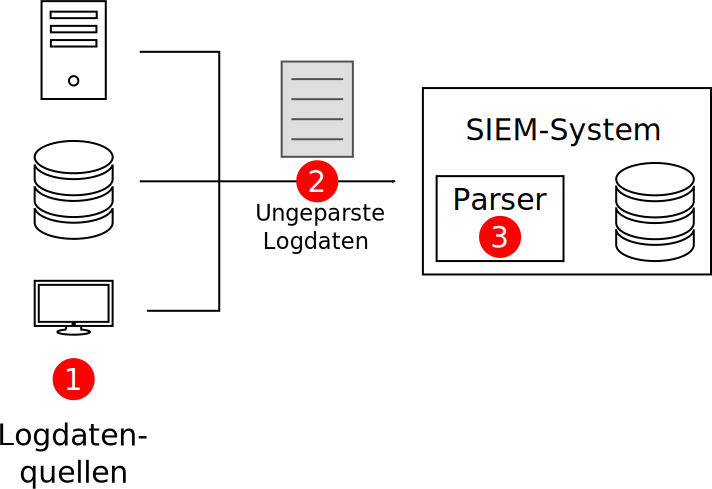
\includegraphics[width=0.5\textwidth]{dia/siem_data_access_point.pdf}
    \caption{Mögliche Eingriffspunkte in den Datenfluss eines SIEM-Systems.}
    \label{fig:siem_data_access_point}
\end{figure}

\begin{enumerate}

\item \textbf{In der Quelle der Logdaten}\\
  Bei diesem Ansatz werden die Daten bereits pseudonymisiert, bevor sie die Datenquelle verlassen. Dieser Ansatz sorgt dafür, dass die Daten bereits pseudonymisiert auf der Übertragungsstrecke und im SIEM-System vorliegen. Es ist kein mehrfaches Parsen der Daten notwendig und der Ansatz ist unabhängig vom verwendeten SIEM-System zu realisieren. Auf der anderen Seite macht der Ansatz die universelle Veränderung jeder Datenquelle notwendig. Dies kann bei Datenquellen, die auf ähnlichen gut erweiterbaren Plattformen beruhen, relativ einfach umzusetzen sein. Beispielsweise könnte die im nächsten Ansatz vorgestellte Proxy-Komponente lokal auf der Datenquelle eingesetzt werden. Schwierigkeiten würde dieser Ansatz hingegen bei Datenquellen bereithalten, die beispielsweise aus Gründen abgespeckter zugrundeliegender Betriebssysteme oder geringer Rechenleistung nur schwer erweiterbar sind. Außerdem würde er in vielen Fällen die Kooperation des Herstellers voraussetzen, wenn es sich um nicht quelloffene \glqq{}Box\grqq{}-Lösungen handelt.

\item \textbf{Proxy-basierter Ansatz}\\
  Dieser Ansatz pseudonymisiert die Daten vor dem ersten Kontakt mit dem SIEM-System, indem Datenquellen ihre Logdaten an einen Proxy senden, der die Daten pseudonymisiert und erst anschließend an das SIEM-System weiterreicht. Hierdurch wird erreicht, dass die Daten zu keiner Zeit nicht-pseudonymisiert in dem SIEM-System vorliegen. Außerdem ist er unabhängig von Datenquellen und SIEM-System und erfordert keinen direkten Eingriff in diese (abgesehen von geringen Konfigurationsanpassungen). Ein Nachteil dieser Lösung ist, dass sie das Parsen und Neuzusammensetzen der Logdaten im Proxy zusätzlich zu deren anschließender Behandlung im SIEM-System erfordert. Außerdem müssen für verschiedene Arten der Logdatenübermittlung (Protokolle wie Syslog oder SNMP) unterschiedliche Proxys entwickelt werden.

\item \textbf{Patchen des SIEM-Systems}\\
  Die letzte Möglichkeit ist das Verändern des SIEM-Systems selbst. Hierzu wird in die Logdaten parsende Komponente eingegriffen, um vor, während oder nach diesem Vorgang die Logdaten zu pseudonymisieren. Dieser Ansatz erfordert kein mehrfaches Bearbeiten von Logdaten wie in dem Proxy-basierten Ansatz. Auf der anderen Seite ist er abhängig vom eingesetzten SIEM-System und erfordert seine Veränderung. Zusätzlich liegen die Daten erst einmal in nicht veränderter Form im SIEM-System vor, was die in Abschnitt \ref{subsec_impl_requirements_ossimintegration} erwähnten Nachteile mit sich bringt.

\end{enumerate}

Aus datenschutztechnischer Sicht ist eine frühestmögliche Pseudonymisierung zu bevorzugen, wie sie auch in \cite{schwartmann2017} empfohlen wird: 
\glqq{}Die Pseudonymisierung ist im Verarbeitungsprozess so früh wie möglich durchzuführen.\grqq{}
Daher wäre eine Pseudonymisierung bereits in der Datenquelle der Optimalfall. Demgegenüber stehen jedoch die erwähnten Nachteile des ersten Ansatzes im Bezug auf die Umsetzbarkeit, da hierzu jede mögliche Quelle von Logdaten universell verändert werden müsste. Eine erst im SIEM-System stattfindende Pseudonymisierung bringt jedoch die beschriebenen Risiken im Bezug auf das Vorliegen des pseudonymisierten Daten im Originalformat mit.

Dies ließ die Entscheidung auf den Proxy-basierten Ansatz fallen. Dass die Lösung außerdem noch keine Anpassungen an dem SIEM-System selbst erfordert, wiegt den Nachteil des zusätzlichen Parsens und wieder Zusammensetzens der Lognachricht bei Weitem auf.
\todo{Auch auf Angreifermodell beziehen?}

\subsection{Architektur}

\label{sec_over_architecture}

%- Wie deckt dieser Ansatz die Anforderungen ab?
%  - Einbindung OSSIM
%  - Pseudonymisierung
%  - Schwellwert
%  - Benutzerinteraktion
%  - Erweiterbarkeit Datenquellen
%  - Erweiterbarkeit Datenschutztechniken

Ausgehend von diesen Überlegungen wurde ein System entworfen, dass die Anforderungen aus Abschnitt \ref{sec_impl_requirements} erfüllt und an der beschriebenen Stelle in den Datenfluss eingreift. 

%\todo{Hier erweitern: Warum verteilte Lsg (ProxyPlugin - Service):
%  - Erweiterbarkeit (Mehrere Proxy-Server mit verschiedenen Protokollen, evtl. auch direkt Client-seitig, ...) => Absicherung einer Komponente, die jedoch auch nicht alles erfährt
%  - Trennung Verarbeitung und Speicherung (Kompr. DB -> Pseudonyme bleiben verdeckt, Kompr. Proxy -> bisherige Daten und Daten evtl. anderer Proxys bleiben abgesichert)
%}

Bei dem Entwurf handelt es sich um ein verteiltes System, bei der die Verarbeitung der Logdaten und die Speicherung der Pseudonymzuordnung an unterschiedlichen Stellen geschieht. Hierfür sprechen verschiedene Gründe. Die Kompromittierung der speichernden Komponente schützt die erstellten Pseudonyme vor Aufdeckung durch die Verschlüsselung der Datensätze mit einem kryptographischen Schwellwertschema. Die Kompromittierung der verarbeitenden Komponente lässt zwar eine Verknüpfung neu erstellter Pseudonyme mit eintreffenden Daten zu, sorgt aber nicht für eine Aufdeckung bereits erstellter Pseudonyme, da diese in der anderen Komponente vorliegen. Weiterhin sorgt dieser Ansatz auch für eine zusätzliche Erweiterbarkeit des Systems. Eine speichernde Komponente kann so als Datenspeicher für mehrere verarbeitende Komponenten agieren, was beispielsweise die Erweiterung um zusätzliche Protokolle (vgl. Abschnitt \ref{sec_impl_integration_into_ossim}) oder Pseudonyme über verschiedene Datenarten (vgl. Abschnitt \ref{sec_state_se_furtherpossibilities}) ermöglicht.
Einen Überblick über den Entwurf bietet Abbildung \ref{fig:high__level_architecture}. Die verschiedenen Komponenten des Systems werden im Folgenden näher beschrieben.

\begin{figure}[]
    \centering
        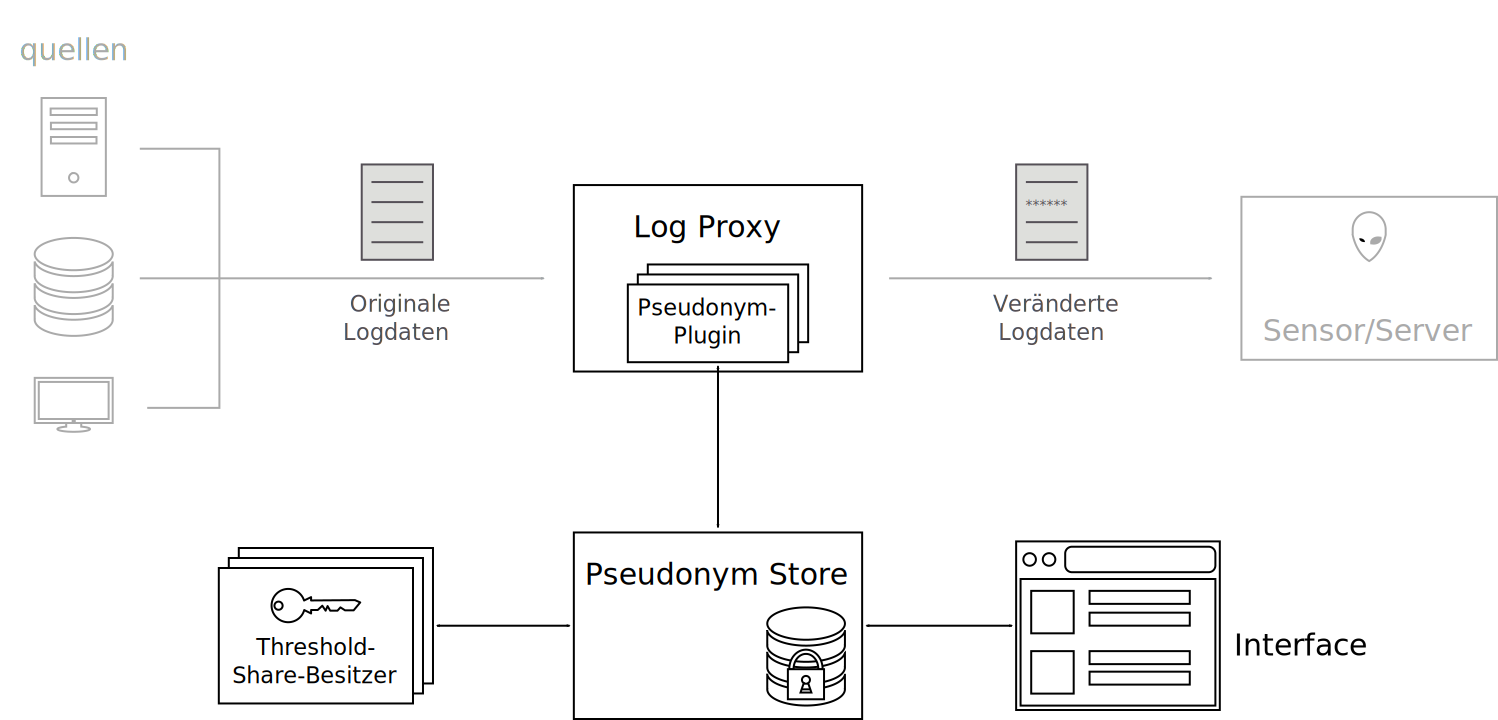
\includegraphics[width=0.9\textwidth]{dia/high_level_architecture.pdf}
    \caption{Ein Überblick über die entworfene Architektur.}
    \label{fig:high__level_architecture}
\end{figure}

Die erste Komponente ist der \textbf{Log-Proxy}, der die Daten entgegennimmt, verändert und anschließend an das SIEM-System weiterleitet. Das Verändern der Daten kann mit verschiedenen Plugins geschehen, so dass neben der umzusetzenden Pseudonymisierung auch weitere Datenschutztechniken eingesetzt werden können, was die geforderte Erweiterbarkeit aus Abschnitt \ref{subsec_impl_requirements_plugins} ermöglicht. Der Proxy leistet die Behandlung von Logdaten aus verschiedenen Quellen wie in Abschnitt \ref{subsec_impl_requirements_differentsources} beschrieben. Das für diese Art des Dateneingriffs erforderliche Parsen und Wiederzusammensetzen der Daten muss hier Datenquellen-abhängig konfigurierbar geschehen.

Ein in dem Proxy enhaltenes Plugin ist für die Pseudonymisierung von Daten zuständig und kommuniziert dazu mit einer externen Komponente -- dem Pseudonym-Service. Die Kommunikation mit dem Proxy erfolgt über einen Webservice-basierten Ansatz. Das Plugin kann für eingehende Daten ein Pseudonym anfordern und dieses anschließend in der Logdatenverarbeitung verwenden.

Der \textbf{Pseudonym-Service} erfüllt zwei Aufgaben: das Speichern und Verwalten der Pseudonyme sowie die Integrierung des kryptographischen Schwellwertschemas. Initial muss die Schlüsselgenerierung des Schwellwertschemas durch den Service geleistet werden. Dies kann wie bereits im vorhergehenden Abschnitt beschrieben zentral oder verteilt geschehen.\\
Es können während des Betriebs neue Pseudonyme angelegt und zusammen mit ihrem durch das Schwellwertschema verschlüsselten Datum abgelegt werden. Sie werden durch geeignete Maßnahmen durchsuchbar gehalten, um für ein Datum überprüfen zu können, ob bereits ein Pseudonym vergeben wurde (dieses Problem wird in Abschnitt \ref{sec_state_se} genauer dargestellt).
Über ein Webinterface kann ein berechtiger Benutzer die Aufdeckung eines bestimmten Pseudonyms fordern und den Status seiner Forderung bzw. im Erfolgsfall das aufgedeckte Datum betrachten. Dieses Datum wird durch das Kombinieren der partiellen Entschlüsselungen erhalten, die von den entsprechenden \textit{Share}-Besitzern berechnet werden. Weiterhin kann über dieses Webinterface auch die initiale Konfiguration des Systems im Bezug auf Eigenschaften des Pseudonymisierung und des kryptographischen Schwellwertschemas vorgenommen werden.\\
Benutzer, die über das Webinterface oder den Webservice mit dem Pseudonym-Service agieren möchten, werden durch geeignete Maßnahmen authentifiziert und ihre Autorisierung überprüft.

Benutzer, die zuständig für die Bewertung von Anfragen zur Aufdeckung eines Pseudonyms sind, erhalten die Möglichkeit zur Interaktion mit dem System über eine \textbf{Client-Anwendung}, für die der Pseudonym-Service ebenfalls als Webservice agiert. Diese Anwendung verwaltet den \textit{Share} des Benutzers für das kryptographische Schwellwertschema und kann nach der Bestätigung des Benutzers zu der Aufdeckung eines Pseudonyms die partielle Entschlüsselung eines Datensatzes erstellen und an den Pseudonym-Service senden.

Für alle Übertragungsstrecken wird angenommen, dass ein Angreifer keinen Zugriff auf Kommunikationsinhalte erhält oder diese verändern kann. Dies ist durch Transportverschlüsselung mittels des weitverbreiteten TLS-Protokolls zu erreichen, muss jedoch bei der Verwendung des Systems beachtete werden. 

\chapter{Stand der Wissenschaft und Auswahl von Verfahren}

In diesem Kapitel soll der aktuelle Stand der Wissenscahft bezogen auf die in dieser Arbeit verwendeten Klassen von Verfahren betrachtet werden sowie ausgehend von den Anforderungen an das zu entwickelnde System ein passendes Verfahren ausgewählt und im Detail beschrieben werden. An geeigneten Stellen wird auf die im letztten Kapitel dargelegten Grundlagen zurückgegriffen.

\label{cha_state}

\section{SIEM-Systeme}

\label{sec_state_siem}

Zur Zeit gibt es eine vielfältige Auswahl an SIEM-Systemen auf dem Markt: Splunk\footnote{
  https://www.splunk.com
}, QRadar von IBM\footnote{
  https://www.ibm.com/us-en/marketplace/ibm-qradar-siem
} oder ArcSight von Micro Focus\footnote{
  https://software.microfocus.com/en-us/software/siem-security-information-event-management
} sind nur einige Beispiele aus diesem Bereich. Neben den in Abschnitt \ref{sec_basics_siem} beschriebenen grundlegenden Funktionen eines SIEM-Systems, die von allen Kandidaten in unterschiedlichem Maße bereitgestellt werden, unterscheiden sie sich insbesondere in darüber hinausgehenden Techniken: Die Nutzung von Machine Learning zur Erkennung ungewöhnlichem Verhaltens oder die Automatisierung von Handlungen im Bedrohungsfall sind hier beispielhafte Möglichkeiten.

Die Auswahl an quelloffener Software in diesem Bereich ist jedoch sehr gering. Eine Ausnahme stellt OSSIM - ein SIEM-System der Firma AlienVault\footnote{
	AlienVault OSSIM: The World’s Most Widely Used Open Source SIEM\\https://www.alienvault.com/products/ossim
} - dar, das auf Basis weiterer quelloffener Lösungen aus dem Netzwerksicherheits-Bereich unter anderem die in Abschnitt \ref{sec_basics_siem} beschriebenen Funktionen bereitstellt. AlienVault bietet zusätzliche eine kommerzielle Variante seines Produkts namens USM an, das insbesondere in den Bereichen Event-Korrelation und Compliance-Reporting die Funktionalität von OSSIM übersteigt. Von der Entwicklungsarbeit die in USM fließt, profitiert jedoch auch OSSIM, beispielsweise durch die Aktualisierung von Plugins für die Einbindung von aktuellen Netzwerkgeräten.

Da die Quelloffenheit auch die Möglichkeit bietet, Komponenten des SIEM-Systems direkt zu verändern, und außerdem gerade im Sicherheitsbereich generell zu bevorzugen ist, fiel die Entscheidung des in dieser Arbeit verwendeten SIEM-Systems auf OSSIM.

\subsection{OSSIM-Überblick}

\label{subsec_state_siem_overview}

Im Folgenden soll eine Übersicht über die für diese Arbeit relevanten Komponenten von OSSIM und deren Zusammenspiel gegeben werden. Diese ist auch in Abbildung \ref{fig:ossim_log_flow} dargestellt.

Den Kern des SIEM-Systems bildet der OSSIM-Server. Hier werden Events gespeichert sowie aggregiert und es findet die Korrelation von Events statt, die der Erkennung von Angriffen oder ungewöhnlichem Netzverhalten dient. Events und generierte Meldungen können über ein Web Interface betrachtet werden. Weiterhin können hier unter anderem Angaben zur Netzinfrastruktur bereitgestellt, Netzwerk- und Schwachstellenscanner bedient und sämtliche Informationen über den Netzwerkstatus eingesehen werden. 

Der OSSIM-Agent ist dafür zuständig, vorliegende Logdaten zu parsen und in ein OSSIM-spezifisches Event-Format zu übersetzen. Auf diesen Vorgang wird im nächsten Abschnitt genauer eingegangen. Die erzeugten Events werden anschließend an den Server weitergeleitet. Der Agent befindet sich sowohl direkt auf dem Server als auch auf jedem installierten Sensor. 

Eine OSSIM-Umgebung kann optional ein oder mehrere Sensoren nutzen, auf denen jeweils ein Agent seine Arbeit verrichtet. Dies wird im Folgenden verteilte Installation genannt. Der Vorteil dieser Lösung besteht darin, dass das aufwendige Parsen und Normalisieren von Logdaten verteilt staffinden und dadurch die Serverlast in großen Umgebungen reduziert werden kann. Kommt kein externer Sensor zum Einsatz, so spricht man von einer All-In-One-Installation.

\begin{figure}[]
    \centering
        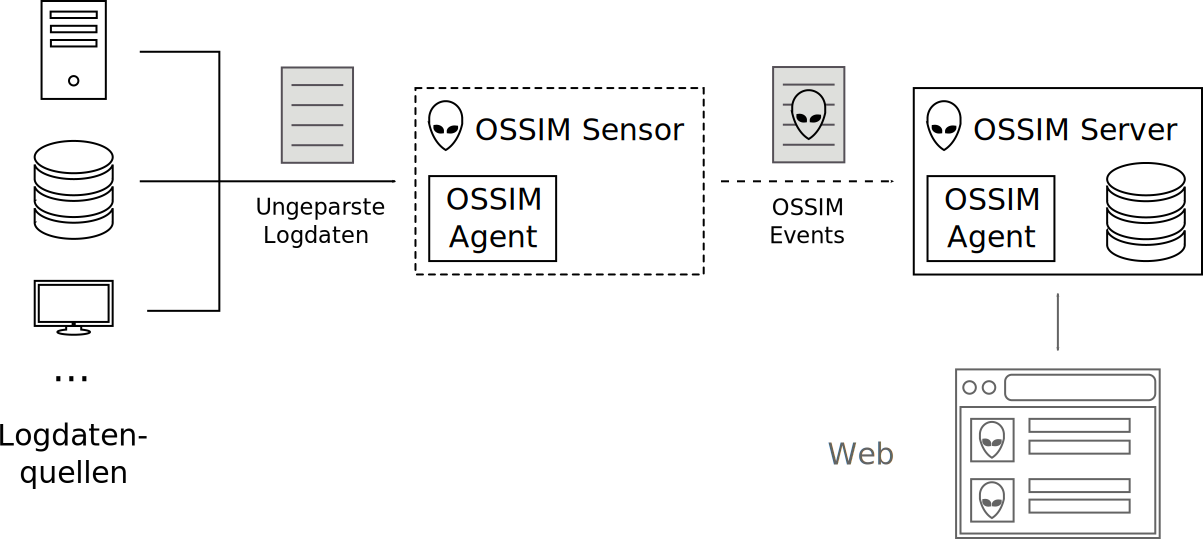
\includegraphics[width=0.9\textwidth]{dia/ossim_log_flow.pdf}
    \caption{High-Level-Übersicht über die OSSIM-Architektur und den Datenfluss.}
    \label{fig:ossim_log_flow}
\end{figure}


\subsection{Parsen von Logdaten in OSSIM}

\label{subsec_state_siem_parsing}

% Quellenarten
% Plugins
% OSSIM-Events
Besonders von Bedeutung für diese Arbeit ist die Verarbeitung von Logdaten. OSSIM ermöglicht es, Logdaten aus unterschiedlichen Quellen entgegenzunehmen bzw. aktiv selber abzurufen und in ein gemeinsames Event-Format zu übersetzen. Hierzu stehen verschiedene Möglichkeiten zur Verfügung:

\begin{itemize}
  \item Entgegennehmen von Daten über das Syslog-Protokoll
  \item Beschaffen von Daten über das SNMP-Protokoll
  \item Entgegennehmen von Daten über proprietäre Protokoll wie SDEE oder WMI
  \item Beschaffen von Daten durch Datenbankabfragen 
\end{itemize}

Unabhängig von der Datenquelle funktioniert die Verarbeitung der Logdaten nach dem immer gleichen Schema. OSSIM bietet die Möglichkeit mitgelieferte oder selber entwickelte Plugins für verschiedene Datenquellen zu aktivieren. Für eintreffende Logdaten überprüft der Agent anhand von regulären Audrücken, ob ein Plugin für das entsprechende Datum zuständig ist. Ist so ein Plugin gefunden, so wird ein neues OSSIM-Event angelegt und anhand der Angaben im Plugin die entsprechenden vorgegebenen Felder des Events gesetzt. Hierbei kann es sich beispielsweise um den Zeitpunkt des Events, IP-Adresse und Port der Datenquelle, einen zu dem Event gehörigen Netzwerkbenutzer oder ereignisabhängige selbstgesetzte Felder handeln. Anschließend folgt die Weiterleitung des Events an den Server.


\section{Pseudonymisierung}

\label{sec_state_pseudonymity}

- A name or another bit string. Identifiers, which are generated using random data only, i.e., fully 
independent of the subject and related attribute values, do not contain side information on the 
subject they are attached to, whereas non-random identifiers may do. E.g., nicknames chosen by 
a user may contain information on heroes he admires; a sequence number may contain 
information on the time the pseudonym was issued; an e-mail address or phone number contains 
information how to reach the user.  \cite{pfitzmann2010}

- evtl. Common Criteria

- VANET

- TIMSI

%pfitzmann2001 - Abschnitt 12
Der Begriff der Pseudonymisierung beschreibt die Benutzung von Pseudonymen zur Identifizierung von Subjekten. Pseudonymisierung sagt dabei erst einmal lediglich etwas über die Verwendung eines Verfahrens aus, jedoch nichts über die daraus entstehenden Auswirkungen auf die Identifizierbarkeit eines Subjekts oder die Zurechenbarkeit bestimmter Aktionen. Hierfür spielen weitere Eigenschaften von Pseudonymen wie die folgenden eine Rolle:
\begin{itemize}
  \item garantierte Eindeutigkeit von Pseudonymen
  \item Möglichkeit von Pseudonymänderungen
  \item begrenzt häufige Verwendung von Pseudonymen 
  \item zeitlich begrenzte Verwendung von Pseudonymen
  \item Art der Pseudonymserstellung
\end{itemize}

Die Ausprägungen dieser Eigenschaften werden auch im Rahmen dieser Arbeit für das umzusetzende System zu bewerten sein.

\section{Schwellwertschemata}

\begin{itemize}
  \item \textbf{Grundlagen} Von Shamirs Secret Sharing bis heute
  \item \textbf{Konkretes Verfahren} Im Detail erläutern - vmtl. Desmedt auf Basis von ElGamal
  \item Zusätzlich Erweiterungen dieses Verfahrens wie verteilte Schlüsselgenerierung.
\end{itemize}

%- Desmedt, Frankel: ElGamal \cite{DesmedtFrankel1990}
%- setzt zentralen "Dealer" voraus
%- Pedersen und verbesserte Variante 
%- Andere Möglichkeiten: Paillier, RSA, ...

\label{sec_state_threshold}

Ein solches System, das auf dem ElGamal-Algorithmus und damit dem Diskreten-Logarithmus-Problem basiert, veröffentlichten die Autoren in \cite{DesmedtFrankel1990}. \todo{Details} Dieser Ansatz setzt in der \textit{Setup}-Phase auf eine zentrale vertrauenswürdige Stelle zur Erzeugung der Schlüssel und \textit{Shares}. In \cite{pedersen1991} stellt der Autor basierend auf diesen Ergebnissen ein Verfahren vor, das bei der Schlüsselgenerierung ohne eine vertrauenswürdige Instanz auskommt. Dieses Verfahren wird in \cite{gennaro1999} noch einmal verbessert.\\
Basierend auf dem jetzigen Recherchestand würde sich diese Kombination von Verfahren gut für den angestrebten Anwendungszweck eignen. Konkrete offene Implementierungen wurden jedoch bisher nicht gefunden, so dass möglicherweise eine eigene Implementierung umgesetzt werden muss.

Neben diesem Verfahren gibt es noch weitere Ansätze basierend auf RSA \cite{desmedt1993, nguyen2005} oder dem Paillier-Kryptosystem \cite{paillier1999, damgard2001}, die jedoch deutlich komplexer zu sein scheinen. 

\todo{TBW}

\section{Searchable Encryption}

\todo{To be written...}

\chapter{Implementierung}

\label{cha_implementation}

\todo{Einführender Absatz}

\section{Einbindung in OSSIM}

\label{sec_impl_integration_into_ossim}

%- Vorgehen
%
%- Nur für Syslog, keine anderen Fomate betrachtet
%
%- Syslog-Nachrichten werden entgegengenommen, geparst und Config-basiert einzelne Datenfelder bearbeitet (basierend auf RegEx)
%
%- Konfigurationsdateien für Datenquellen (leichte Erweiterbarkeit, auch im Bezug auf neue Datenquellen, ...) mit Beispiel
%
%- Plugins (leichte Erweiterbarkeit, ...)

\todo{Proxy-Aufbau und Vorgehensweise erläutern, insgesamt Abschnitte besser verknüpfen}


Für die in dieser Arbeit zu leistende prototypische Umsetzung des Systems wurde sich auf den am häufigsten\footnote{
  Die in OSSIM bereits mitgelieferten Plugins bestätigen dies. Unter den Hunderten Plugins ist nur ein einziges, das einen anderen Mechanismus als das Syslog-Protokoll nutzt. Auch wenn beispielsweise Plugins, die eine Datenbankabfrage enthalten, immer dem Anwendungsfall angepasst und daher nicht in OSSIM inkludiert werden können, so unterstützt dies doch die Annahme des Syslog-Protokolls als am häufigsten genutzten Weg und damit als geeignet für den Fokus dieser Arbeit.
} genutzten Weg des Datenerhalts in OSSIM (siehe Abschnitt \ref{subsec_state_siem_parsing}) beschränkt: das Entgegennehmen der Daten über das Syslog-Protokoll. 




Die Behandlung von verschiedenen Datenquellen wird durch Konfigurationsdateien ermöglicht:

\begin{lstlisting}[morekeywords={general,active,pattern,group1,group2}]
[general]
active=True

[group1]
pattern=^(?P<time>\w+ *\d{1,2} \d{2}:\d{2}:\d{2}) (?P<device>[^:]+): Testing my device USER=(?P<user>.+)$
time=Substitute(substitute = 'somevalue_time')
device=Substitute(substitute = 'somevalue_device')
user=Pseudonymize()

[group2]
pattern=^(?P<test>.*)$
test=Pseudonymize()
\end{lstlisting}

Eine Konfigurationsdatei kann aus mehreren Bereichen bestehen. Der \texttt{general}-Bereich enthält allgemeine Angaben über das Plugin. Um unterschiedliche Lognachrichten eines Gerätes bündeln zu können, kann eine Konfigurationsdatei weiterhin mehrere Bereiche enthalten, die jeweils die Verarbeitung einer bestimmten Lognachricht beschreiben. Angegeben werden muss jeweils ein regulärer Audruck, der die Nachricht beschreibt und mehrere Gruppen (\texttt{(?P<name>...)}) enthalten kann. Für jede dieser Gruppen muss eine Angabe zu dem Plugin inklusive notwendiger Parameter gemacht werden, dass die Gruppe verarbeiten soll. Durch diese Konfigurationsdateien können Nachrichten unbekannter Formate aus neuen Datenquellen leicht in das bestehende System eingebunden werden.



Die Erweiterbarkeit um neue Datenschutztechniken wird durch leicht erweiterbare Plugins ermöglicht. Ein Plugin muss lediglich die Methode \texttt{handle\_data} implementieren, die die originalen Daten und alle in der Konfiguration angegebenen Parameter erhält. Ein einfaches Plugin, das die Daten durch ein in der Konfiguration angegebenen Wert ersetzt, könnte so aussehen:

\begin{lstlisting}[language=Python]
class Substitute(AbstractPlugin):

    def handle_data(self, data: str, **kwargs) -> str:
        if 'substitute' in kwargs:
            return kwargs['substitute']
        else:
            raise MissingSubstituteError
\end{lstlisting}

\section{Umsetzung der Pseudonymisierung} % und Searchable Encryption

\label{sec_impl_pseudonymity}

% Pseudonymgenerierung

% Parameter: Zeitabhängig, Häufigkeitsabhängig, USE_PFP
% Wie erfolgt die Konfiguration? Wo werden Werte gesetzt/gespeichert?

% MAC Generierung (bzw. Empfang als Search_token) beschreiben

% Zweiter MAC?
% Auch auf Vertrauensmodell im Zusammenhang mit PFP eingehen: Was erfährt die DB, was lässt sich verketten, was würde bei Aufdecken eines Pseudonyms geschehen? Was passiert bei unerlaubtem Zugriff auf gespeicherte Daten?


Für die Pseudonymisierung wurde ein Plugin für den Proxy entwickelt. Bei jedem eintreffenden Logdatum kann abhängig von dem Datenformat für ein entsprechendes Datenfeld ein Pseudonym als Ersatz für das echte Datum gesetzt werden. Dazu stellt der Pseudonym-Service eine Schnittstelle bereit, über die für ein Datum ein Pseudonym erhalten werden kann. Durch diese Trennung wird eine höhere Sicherheit der Zuordnung zwischen Datum und Pseudonym erreicht: In dem Proxy kommen die Logdaten in unveränderter Form an und werden verändert weitergesendet, daher ist die Zuordnung hier implizit bekannt und muss in Kauf genommen werden. Die Speicherung dieser Zuordnung erfolgt jedoch nur in dem Pseudonym-Service. Durch die Verschlüsselung und die in den folgenden Abschnitten beschriebene MAC-abhängige Pseudonymgenerierung erfährt der Pseudonym-Service nichts über das Datum, das durch das Pseudonym beschrieben wird. So führt unberechtigter Zugriff auf die Datenbank des Pseudonym-Service nicht zu mehr Informationen über das Datum, das ein Pseudonym bescchreibt.

Auf der Proxy-Seite wird das verschlüsselte Datum (siehe dazu Abschnitt \ref{sec_impl_threshold}) zusammen mit einem generierten MAC, der wie in Abschnitt \ref{sec_state_se} beschrieben für die Überprüfung auf bereits bestehende Pseudonyme genutzt wird, an den Pseudonym-Service gesendet. 
Der Schlüssel, der für die Generierung des MACs verwendet wird, wird immer nach einer bestimmten Zeitspanne neu generiert. Diese Zeitspanne kann mittels eines Parameters an das Anwendungsszenario angepasst werden (vgl. \ref{sec_state_pseudonymity}). Durch diesen Schlüsselwechsel wird erreicht, das für gleiche Daten, für die der MAC mit einem neuen Schlüssel erstellt wird, auch neue Pseudonyme erhalten werden. \\
Da der Schlüsselwechsel nicht Pseudonym-abhängig geschieht, ist die Zeitspanne global für alle Pseudonyme gültig und somit als maximale Zeitspanne zu verstehen. Dies kann für die Anomalieerkennung evtl. Probleme bereiten, wenn nicht genügend lange Überwachungsdaten verkettet werden können. Auf der anderen Seite würde eine Verweildauer für einzelne Pseudonyme ein Erfassen des Erstellungszeitpunkts in der Datenbank erfordern, was wie in Abschnitt \ref{sec_state_pseudonymity} beschrieben Rückschlüsse auf das ursprüngliche Datum des Pseudonyms liefern könnte. Daher wurde sich gegen diesen Ansatz entschieden.

Auf der Service-Seite wird nun anhand des empfangenen MACs durch Vergleich mit in der Datenbank vorliegenden MACs überprüft, ob bereits ein Pseudonym für das Datum vergeben wurde, das noch nicht zu häufig verwendet wurde. Ist dies noch nicht der Fall, so wird ein noch nicht verwendetes, zufälliges Pseudonym erstellt und zusammen mit dem MAC in der Datenbank gespeichert. Anderenfalls wird das bereits vergebene Pseudonym zurückgeliefert. Die maximale Anzahl an Nutzungen kann analog zur maximalen Zeitspanne ebenfalls mittels eines Parameter gesetzt werden. 

Im Zusammenspiel dieser Parameter kann jedoch noch ein Problem entstehen. Für neu vergebene Pseudonyme, die innerhalb eines Zeitabschnitts durch Überschreiten der maximalen Nutzungsanzahl entstanden sind, liegen in der Datenbank Einträge mit gleichem MAC vor. So wird die Verknüpfung verschiedener Pseudonyme ermöglicht, wenn jemand (berechtigt oder unberechtigt) Zugriff auf die Daten erhält. Das Aufdecken eines Pseudonyms deckt auch alle anderen in diesem Zeitintervall erstellten Pseudonyme implizit auf, was dem in Abschnitt \ref{sec_state_pseudonymity} beschriebenen Prinzip der \textit{Perfect Forward Privacy} widerspricht. 
Dieses Problem kann durch eine zusätzliche MAC-Berechnung auf der Service-Seite verhindert werden, die zusätzlich noch einen Pseudonym-abhängigen Zufallswert einbeziehen muss. Der hierzu verwendete Schlüssel muss dann ebenfalls abhängig von dem bereits beschriebenen Parameter neu generiert werden. Hierdurch enthalten Datenbankeinträge, die innerhalb eines Zeitintervalls zu dem gleichen Datum gehören, durch den einfließenden Zufallswert trotzdem unterschiedliche MACs und die Verkettbarkeit verschiedener Pseudonyme ist verhindert. Jedoch erfordert dieser Ansatz eine MAC-Berechnung pro Datenbankeintrag für jede Anfrage und ist daher aus Performance-Sicht kritisch zu betrachten. Daher wird diese Möglichkeit nicht implementiert. Das bestehende Problem ist jedoch für ein konkretes Anwendungsszenario und bei der Wahl der Parameter -- insbesondere des Zeitintervalls -- zu beachten.


\section{Implementierung und Integration des Schwellwertschemas}

\label{sec_impl_threshold}

Something

\subsection{ThresholdCrypto \glqq Lib\grqq{}}

- Bibliothek, die statuslos in allen Teilen des Systems verwendet werden kann.

- Interface

  \subsubsection{Parametergenerierung}
  
  - Verwendete Gruppen und Auswirkungen fester Parameter? HoC, ...
  
  \subsubsection{Hybride Kryptographie}
  
  - Erzeugung symmetrischer Schlüssel und symmetrische Kryptographie per NaCl(pynacl) -> Authenticated Encryption ChaCha Salsa
  
  - lediglich Verschlüsselung dieses Schlüssels mit dem Schwellwertschema
  
  - von erfahrenen Kryptographen entwickelt
  - getestet
  - schnell
  - Beliebiger Nachrichteninhalt ohne Auswirkungen auf die Verschlüsselung

\subsection{Setup-Verfahren}

auf bereits in impl-pseudonymity geschriebenes zurückgreifen

\subsection{Client-Anwendung}

- Shares empfangen und verschlüsselt abspeichern

- Enthält Webserver um Shares niemals auf dem Server speichern zu müssen

\subsection{Proxy}

- Empfängt PublicKey vom Service und nutzt ihn zur Nachrichtenverschlüsselung




\section{Evaluation}

\label{sec_impl_evaluation}

\subsection{Erfüllung der Anforderungen}

\begin{itemize}
  \item Geeignete Stelle zum Eingriff in den Datenfluss zwischen Logdatenquelle und SIEM-System
  \item Parameterabhängige Generierung eindeutiger, aber in gewissem Rahmen verknüpfbarer Pseudonyme
  \item Sicherer, verteilter Einsatz eines anpassbaren kryptographischen Schwellwertschemas -- vorzugsweise mit verteilter Schlüsselgenerierung
  \item Geeignete Benutzerinteraktion mit dem System an notwendigen Stellen
  \item Erweiterbarkeit um unbekannte Datenquellen
  \item Erweiterbarkeit um weitere Datenschutztechniken
\end{itemize}

...

\subsection{Angriffsmöglichkeiten}

- Zentrale Schlüsselgenerierung (Verweis auf state-distributed)

- Krypto nicht von Kryptographen überprüft (Sidechannel, ...)

- Mögliche Schwächen (sowohl Architektur als auch Krypto, Bezug zum Angreifermodell)

- Scheme leakt Nachrichtenlänge als Vielfaches der Blocklänge -> Paddingscheme?

- Reidentification-Problem (siehe auch Lundin 4.3)

\subsection{Performance}

- Zeitmessungen für einzelne Systemfunktionen

- Performance bzw. Auswirkungen der Nutzung (theoretische Rechenlast, Zeit-/Lastmessung, zusätzlicher Speicherbedarf, ...)
















\chapter{Alternativen}

\begin{itemize}
  \item \textbf{Alternativen} Welche alternativen oder ergänzenden Vorgehensweisen zu Pseudonymisierung + kryptographisches Schwellwertschema gibt es und welche Eigenschaften, Vor- und Nachteile besitzen sie?
  \item \textbf{Umsetzung} Wie könnten diese Alternativen im Prototypen umgesetzt werden?
\end{itemize}

% Generalisierung (zb nur noch Abteilung betrachten)
% Löschung
% Rauschen hinzufügen zB Zeitstempel plus normalverteilten Zufallswert (Christian)
% ...
%

\label{cha_alternatives}

\section{Alternative1}

\section{...}

\section{Vorgehen zur Integration}

\chapter{Fazit}

\label{cha_final}

\todo{TBW}

% ================================Literature==============================

\begin{raggedright}         % Schaltet Blocksatz ab, erzeugt ein stimmigeres
                            %  Schriftbild im Literaturverzeichnis.
  \printbibliography        % Falls Biblatex verwendet wird.
  \label{sec:literaturverzeichnis}
\end{raggedright}

\newpage
\pagenumbering{gobble}

\chapter*{Eidesstattliche Versicherung}

Hiermit  versichere  ich  an  Eides  statt,  dass  ich  die  vorliegende  Arbeit  im 
Masterstudiengang  Informatik  selbstständig  verfasst  und  keine  anderen  als  die 
angegebenen  Hilfsmittel  --  insbesondere  keine  im  Quellenverzeichnis  nicht 
benannten  Internet-Quellen  --  benutzt  habe.  Alle  Stellen,  die  wörtlich  oder 
sinngemäß aus Veröffentlichungen entnommen wurden, sind als solche kenntlich 
gemacht. Ich versichere weiterhin, dass ich die Arbeit vorher nicht in einem anderen 
Prüfungsverfahren eingereicht habe und die eingereichte schriftliche Fassung der 
auf dem elektronischen Speichermedium entspricht.

Ich stimme der Einstellung der Arbeit in die Bibliothek des Fachbereichs Informatik 
zu.

\vspace{1cm}

Hamburg, der 23. März 2018

\vspace{3cm}

\par\noindent\rule{0.3\textwidth}{0.4pt}

Tom Petersen

\end{document}

